\documentclass[12pt,prb,aps]{revtex4-1}
\usepackage {amsmath}
\usepackage{amssymb}
\pdfoutput = 1 
\usepackage {graphicx}
\newcommand{\bomega}{\mbox{\boldmath$\omega$}}


\begin{document}

\title{Multi-Harmonic Rutherford Island Theory}

\author{R.~Fitzpatrick\,\footnote{rfitzp@utexas.edu}}
\affiliation{Institute for Fusion Studies,  Department of Physics,  University of Texas at Austin,  Austin TX 78712, USA.}

\begin{abstract}
Rutherford island theory, which governs the nonlinear evolution of tearing modes in tokamak plasmas,  is generalized to take into account situations in which the conventional one-harmonic
approximation is not valid. The analysis incorporates  non-inductive currents driven by radio-frequency (RF) electromagnetic waves injected into the plasma. A
multi-harmonic tearing mode dispersion relation is derived that takes the form of a nonlinear inhomogeneous matrix
eigenvalue problem.   The  dispersion relation is solved in the so-called two-harmonic approximation,
in which  only the principal Fourier harmonic of the perturbed magnetic flux and its first overtone are included in the calculation.
In the absence of RF current drive, the nonlinear behavior of a tearing
mode predicted in the two-harmonic approximation does not differ substantially from that predicted in the
 one-harmonic approximation.  On the other hand, RF current drive that is sufficiently localized in the
vicinity of the O-points of the mode's magnetic island chain is capable of triggering  homoclinic bifurcations of the O-points (which is impossible in the one-harmonic approximation). However, current
drive is incapable of triggering heteroclinic bifurcations of the island X-points. This is significant because
 Bard\'{o}czi \& Evans [Phys.\ Rev.\ Lett.\ {\bf 126}, 085003 (2021)]  observed homoclinic bifurcations of magnetic island chains in the presence of RF
 current drive in the DIII-D tokamak, but did not observe heteroclinic bifurcations. Finally, the changes in topology of the magnetic island
 flux-surfaces induced by RF current drive are found to facilitate the stabilization of the tearing mode. 
\end{abstract}

\maketitle

\section{Introduction}
Tearing modes are magnetohydrodynamical  (MHD) instabilities that often limit fusion plasma performance in  magnetic confinement devices, such as tokamaks, that rely on nested toroidal
magnetic flux-surfaces.\cite{fkr,wesson} As the name suggests, ``tearing''
modes tear and reconnect magnetic field-lines, in the process
converting nested toroidal flux-surfaces into helical magnetic
island chains.\cite{ruth} Such island chains degrade plasma confinement because
heat and particles are able to travel radially from one side of
the chain to the other by flowing along magnetic field-lines,
which is a relatively fast process, instead of having to diffuse
across magnetic flux-surfaces, which is a relatively slow
process, giving rise to a flattening of the plasma pressure across the  chain.\cite{chang,fitz}

{\em Classical tearing modes}\/ are driven by current gradients within the plasma.\cite{fkr} However,
so-called {\em neoclassical tearing modes}\/ (NTMs) are driven by the loss of the {\em bootstrap current}, which is a non-inductive current induced by plasma pressure gradients,\cite{boot} as a consequence of  the
flattening of the pressure gradient across the associated magnetic island chain.\cite{carrera}
NTMs in tokamaks are the main limitation to the achievement of an adequate level of normalized plasma pressure for the
purposes of thermonuclear fusion.\cite{buttery}
NTMs are usually controlled in tokamaks by means of an additional non-inductive current driven in the immediate
vicinity of the island chain via radio-frequency (RF) electromagnetic waves injected into the plasma.\cite{buttery,lahaye} The purpose of the RF current
drive is to replace the missing bootstrap current within the island chain, and, thereby, to stabilize the
 mode.\cite{westerhof} It should be noted, however, that RF current drive can also be used to
 stabilize classical tearing modes.\cite{westerhof}
 
 The nonlinear growth of tearing modes is described by a theory that was first published almost 50 years ago by Rutherford.\cite{ruth} According to Rutherford's theory:
 \begin{enumerate}
 \item Linear analysis becomes invalid as soon as the width of the magnetic island chain exceeds the linear layer width.
 Given that the linear layer widths in high temperature tokamak plasmas are very thin (i.e., typically a factor $S^{-2/5}$
 smaller than the minor radius, where $S\gtrsim 10^8$ is the Lundquist number),\cite{fkr} it follows that if a tearing mode has attained a sufficient amplitude to be detectable experimentally then it is already in the nonlinear regime. 
 \item As soon as the island width exceeds the linear layer width,  inertia becomes negligible in the
 plasma equation of motion.  The absence of inertia in the equation of motion also
 forces the plasma current density to be constant on  each magnetic flux-surface of the island chain. 
 \item Assuming that the tearing mode is not too unstable, the constant-$\psi$ approximation can be employed in the
 immediate vicinity of the island chain.\cite{fkr} This enables a simple analytic solution for the island magnetic flux-surfaces. 
 \item Given that the island flux-surfaces are known, and that the current density is a flux-surface function, plasma
 flow can be eliminated from the plasma Ohm's law, by means of a suitable flux-surface average operator, to determine the
 current density profile in the immediate vicinity of the island chain.
 \item The current density profile in the immediate vicinity of the island chain can be used to asymptotically match
 the island solution to a conventional tearing mode solution, 
governed by 
 linear ideal-MHD,  in the remainder  of the plasma to produce a tearing mode dispersion relation. According to this dispersion
 relation, the width of the island chain grows {\em linearly}\/ in time.
 \item The current density profile in the vicinity of the island chain contains multiple harmonics. In other words,
 if we are talking about a tearing mode in a tokamak that creates an island chain with $m_\theta$ periods in the poloidal direction, and $n_\phi$ periods in the
 toroidal direction, then the current density in the island region has a ($m_\theta$, $n_\phi$) component, but also a  ($2\,m_\theta$, $2\,n_\phi$) component, and a ($3\,m_\theta$, $3\,n_\phi$) component, et cetera. Nevertheless, the
 perturbed magnetic field in the island region is assumed to be dominated by the ($m_\theta$, $n_\phi$) component. Henceforth, we shall refer to this assumption as the {\em one-harmonic approximation}. 
 \end{enumerate}
 
A recent experimental paper by Bard\'{o}czi \& Evans\,\cite{bar} clearly shows that the one-harmonic
approximation is not necessarily valid, especially in cases in which RF-driven non-inductive
currents  are applied in the island region. 
The purpose of this paper is to examine under which circumstances the one-harmonic approximation is valid, and
also to devise a multi-harmonic extension to Rutherford's analysis that is capable of  describing situations in 
which the one-harmonic approximation fails. 

In this paper, for the sake of simplicity, we shall perform our analysis
in slab geometry. However, the generalization to cylindrical geometry is straightforward. We shall also restrict our attention to classical tearing modes interacting with RF-driven non-inductive currents. The incorporation of the
bootstrap current into the analysis is also straightforward (it is just an addition non-inductive current). 

\section{Preliminary Slab Analysis}
\subsection{Reduced-MHD Equations}
Our starting point is a set of MHD equations that neglects plasma compressibility,
but incorporates  plasma resistivity and non-inductive current drive: 
\begin{align}
\nabla\cdot{\bf V} &= 0,\label{e9.1m}\\[0.5ex]
\rho\left[\frac{\partial {\bf V}}{\partial t} + ({\bf V}\cdot\nabla) {\bf V}\right]+\nabla p-{\bf j}\times {\bf B} &=0,\label{e9.2m}\\[0,5ex]
{\bf E} + {\bf V} \times {\bf B} &=\eta\,({\bf j}-{\bf j}_{\rm ni}).\label{e9.3m}
\end{align}
Here, ${\bf V}$, $p$,   ${\bf j}$, ${\bf j}_{\rm ni}$, ${\bf B}$,  and ${\bf E}$  represent the plasma flow velocity, the plasma
pressure, the total plasma current density, 
the non-inductive component of the plasma current density, the magnetic field-strength, and the electric field-strength, respectively.  Moreover, the plasma mass density, $\rho$, and resistivity, $\eta$, are both assumed to be spatially uniform, for the sake of simplicity.  
Equations (\ref{e9.1m})--(\ref{e9.3m})  form a complete set when combined with the following subset of 
Maxwell's equations:
$\nabla\cdot{\bf B} =0$,
$ \nabla\times {\bf E}=-\partial{\bf B}/\partial t$, and $\nabla\times {\bf B} = \mu_0\,{\bf j}$.
 
Consider a simplified slab scenario in which the Cartesian coordinate $z$ is ignorable. In other words, there is
no variation in the $z$-direction (i.e., $\partial/\partial z=0$). We can automatically satisfy Eq.~(\ref{e9.1m})
and $\nabla\cdot{\bf B} = 0$ by writing
${\bf V} =\nabla\phi\times {\bf e}_z + V_z\,{\bf e}_z$ and 
${\bf B} = \nabla\psi\times{\bf e}_z + B_z\,{\bf e}_z$,
where ${\bf e}_z$ is a unit vector parallel to the $z$-axis, and $V_z$ and $B_z$  are constants.  

If we take the $z$-component of Eq.~(\ref{e9.3m}) and the $z$-component of the curl of Eq.~(\ref{e9.2m}), making use of Maxwell's equations,
then we obtain the  so-called {\em reduced-MHD equations}:\,\cite{strauss}
\begin{align}
\frac{\partial\psi}{\partial t} &= [\phi,\psi]+\frac{\eta}{\mu_0}\,(J-J_0-J_{\rm ni}),\label{e9.11m}\\[0.5ex]
\rho\,\frac{\partial U}{\partial t} &= \rho\,[\phi,U] + \mu_0^{-1}\,[J,\psi],\\[0.5ex]
J&=\nabla^2\psi,\\[0.5ex]
U&=\nabla^2\phi,\label{e9.14m}
\end{align}
where $[A,B]\equiv \nabla A\times \nabla B\cdot{\bf e}_z$. Here, the plasma current density
is written ${\bf j} = -\mu_0^{-1}\,J\,{\bf e}_z$, the  non-inductive current density is written ${\bf j}_{\rm ni} = -\mu_0^{-1}\,J_{\rm ni}\, {\bf e}_z$, 
 and $\bomega\equiv \nabla\times{\bf V}=-U\,{\bf e}_z$ is the plasma vorticity. 
Moreover, $J_0(x)=-(\mu_0/\eta)\,E_{z\,{\rm in}}$, where $E_{z\,{\rm in}}(x)$ is  the $z$-directed inductive electric field that maintains the equilibrium current density.

\subsection{Linearized Reduced-MHD Equations}
Consider the stability of a current sheet whose equilibrium state is characterized by zero flow and 
\begin{align}
{\bf B}&= B_0\,F(x/a)\,{\bf e}_y,\\[0.5ex]
{\bf j}&= \frac{B_0}{\mu_0\,a}\,F'(x/a)\,{\bf e}_z,
\end{align}
where $F(-y)= - F(y)$, $F(y)\rightarrow {\rm sgn}(y)$ as $|y|\rightarrow 1$, and $'$ denotes differentiation with
respect to argument.  Here, $a$ is a measure of the thickness of the sheet, and $B_0$ is a typical value of $B_y$ within the sheet.   (So, in tokamak geometry, $a$ represents the minor radius, and $B_0$ is the typical
poloidal magnetic field-strength.) Neglecting the non-inductive current
drive, for the moment, 
 we  deduce from Eq.~(\ref{e9.11m}) that
\begin{equation}
J_0(x) = - \frac{B_0}{a}\,F'(x/a).
\end{equation}

Suppose that the system is periodic in the $y$ direction, with period $L$. (In tokamak geometry, $L=2\pi\,r_s/m_\theta$ where $r_s$ is the minor radius of the resonant surface.) Consider a small-amplitude perturbation to the system of the
form
\begin{align}\label{e11}
\psi(x,y,t) &= -B_0\int_0^xF(x'/a)\,dx' + \sum_{m=1,\infty}\psi_m(x)\,{\rm e}^{\,{\rm i}\,(m\,k_0\,y+\gamma\,t)},\\[0.5ex]
J(x,y,t) &= -\frac{B_0}{a}\,F'(x/a)+ \sum_{m=1,\infty}J_m(x)\,{\rm e}^{\,{\rm i}\,(m\,k_0\,y+\gamma\,t)},\\[0.5ex]
\phi(x,y,t) &=  \sum_{m=1,\infty}\phi_m(x)\,{\rm e}^{\,{\rm i}\,(m\,k_0\,y+\gamma\,t)},\\[0.5ex]
U(x,y,t) &=  \sum_{m=1,\infty}U_m(x)\,{\rm e}^{\,{\rm i}\,(m\,k_0\,y+\gamma\,t)},\label{e14}
\end{align}
where $k_0=2\pi/L$. (In tokamak geometry, $k_0\,y = m_\theta\,\theta-n_\phi\,\phi$, where $\theta$ and $\phi$
are the poloidal and toroidal angles, respectively.)

Substituting Eqs.~(\ref{e11})--(\ref{e14}) into the reduced-MHD equations, (\ref{e9.11m})--(\ref{e9.14m}), and
only retaining terms that are first order in small quantities, we obtain the so-called {\em linearized reduced-MHD equations}: 
\begin{align}
\gamma\,\psi_m &= {\rm i}\,k_m\,B_0\,F\,\phi_m +\frac{\eta}{\mu_0}\left(\frac{d^2}{dx^2}-k_m^{2}\right)\psi_m,\label{e15}
\\[0.5ex]
\gamma\,\rho\left(\frac{d^2}{dx^2}-k_m^{2}\right)\phi_m &= {\rm i}\,\mu_0^{-1}\,k_m\,B_0\,F\left(\frac{d^2}{dx^2}
-k_m^{2}-\frac{F''}{a^2\,F}\right)\psi_m,\label{e16}
\end{align}
where $k_m= m\,k_0$. 

It is helpful to define the Alfv\'{e}n timescale,
\begin{equation}
\tau_{A\,m} = \frac{k_m^{-1}}{(B_0^{\,2}/\mu_0\,\rho)^{1/2}},
\end{equation}
the resistive diffusion timescale,
\begin{equation}
\tau_R = \frac{\mu_0\,a^2}{\eta},
\end{equation}
and the Lundquist number,
\begin{equation}
S_m = \frac{\tau_R}{\tau_{A\,m}}.
\end{equation}
It is assumed that $S_m\gg 1$. 

Let $x=a\,\hat{x}$, $k_m = \hat{k}_m/a$, $\gamma=\hat{\gamma}/\tau_{A\,m}$, $\psi_m = -a\,B_0\,\hat{\psi}_m$,
and $\phi_m= {\rm i}\,(\gamma\,a/k_m)\,\skew{3}\hat{\phi}_m$. The dimensionless normalized versions of the
linearized reduced-MHD equations, (\ref{e15}) and (\ref{e16}),  become
\begin{align}
S_m\,\hat{\gamma}\left(\hat{\psi}_m-F\,\skew{3}\hat{\phi}_m\right)&= \left(\frac{d^2}{d\hat{x}^2}-\hat{k}_m^2\right)\hat{\psi}_m,\label{e9.27}\\[0.5ex]
\hat{\gamma}^{\,2}\left(\frac{d^2}{d\hat{x}^2}-\hat{k}_m^2\right)\skew{3}\hat{\phi}_m&= - F\left(\frac{d^2}{d\hat{x}^2}
-\hat{k}_m^2-\frac{F''}{F}\right)\hat{\psi}_m.\label{e9.28}
\end{align}
 Our normalization scheme is designed such that, throughout the
bulk of the plasma, $\hat{\psi}_m\sim \skew{3}\hat{\phi}_m$, and the only other quantities in the previous two equations whose magnitudes differ substantially
from unity are $S_m\,\hat{\gamma}$ and $\hat{\gamma}^{\,2}$. 

\subsection{Asymptotic Matching}
Suppose that the perturbation   grows on a timescale that is much less than $\tau_R$, but much greater than
$\tau_{A\,m}$. It follows that
\begin{equation}\label{e9.29}
\hat{\gamma} \ll 1 \ll S_m\,\hat{\gamma}.
\end{equation}
Thus, throughout the bulk of the plasma, we can neglect the right-hand side of Eq.~(\ref{e9.27}), and the left-hand side of Eq.~(\ref{e9.28}), which is equivalent to the neglect of plasma resistivity and inertia. In this case,
Eqs.~(\ref{e9.27}) and (\ref{e9.28}) reduce to the so-called {\em linearized marginally-stable ideal-MHD equations}:
\begin{align}
\skew{3}\hat{\phi}_m &= \frac{\hat{\psi}_m}{F},\label{e9.30}\\[0.5ex]
\frac{d^2\hat{\psi}_m}{d\hat{x}^2} - \hat{k}_m^2\,\hat{\psi}_m-\frac{F''}{F}\,\hat{\psi}_m &= 0.\label{e9.31}
\end{align}
Equation~(\ref{e9.30}) is equivalent to the well-known {\em flux-freezing constraint},\cite{fried} and forbids any changes in the
topology of the equilibrium magnetic field-lines. 
However, it is clear that the linearized marginally-stable ideal-MHD  equations break down in the
immediate vicinity of the so-called {\em resonant surface}, located at $x=0$,  where $F=0$ (i.e., where $B_y$ reverses direction). This follows from Eq.~(\ref{e9.30}), which implies that $\skew{3}\hat{\phi}_m\rightarrow\infty$ as $F\rightarrow 0$ if $\hat{\psi}_m(0)\neq 0$ (i.e., if the topology of the magnetic
field-lines changes in the  vicinity of the resonant surface). [In tokamak geometry, the resonant surface is located at
minor radius $r=r_s$, where 
$q(r_s)=m_\theta/n_\phi$. Here, $q(r)=r\,B_\phi/(R_0\,B_\theta)$ is the safety-factor profile, $B_\theta$ is the 
equilibrium poloidal magnetic field, and $B_\phi$ is the equilibrium toroidal magnetic field.\cite{wesson}]
 In general, we need to employ the full set of reduced-MHD equations in the so-called {\em inner region}, close to the resonant
surface, where Eqs.~(\ref{e9.30}) and (\ref{e9.31}) break down. The remainder of the plasma,
which is governed by the linearized marginally-stable ideal-MHD  equations, is known as the {\em outer region}. 

The stability problem reduces to solving the  reduced-MHD equations, (\ref{e9.11m})--(\ref{e9.14m}), in the inner region, solving the linearized marginally-stable ideal-MHD
equations, (\ref{e9.30}) and (\ref{e9.31}), in the outer region, and matching the two solutions at the boundary between the
inner and outer regions.\cite{fkr} In general, the tearing-parity [i.e., $\hat{\psi}_m(-\hat{x})=\hat{\psi}_m(\hat{x})$] solution of the so-called {\em tearing mode equation,} (\ref{e9.31}), that satisfies
physical boundary conditions at $|\hat{x}|\rightarrow\infty$ (i.e., $|\hat{\psi}_m|\rightarrow 0$ as $|\hat{x}|\rightarrow \infty$), has a gradient discontinuity across the resonant surface.\cite{fkr} 
Note that the adopted boundary conditions assume that the plasma is isolated. In other words, the plasma is not subject to any externally generated magnetic perturbations. It is helpful to define the {\em tearing stability
index},\cite{fkr} 
\begin{equation}\label{e25}
{\mit\Delta}_m' =\left[\frac{1}{\hat{\psi}_m}\,\frac{d\hat{\psi}_m}{d\hat{x}}\right]_{\hat{x}=0_-}^{\hat{x}=0_+}.
\end{equation}
This real dimensionless quantity is uniquely determined by the tearing mode equation, and the boundary conditions,
for each mode number, $m$. 

Let $W_1\ll a$ be the thickness (in $x$) of the inner region. Our task is thus to solve the   reduced-MHD equations, (\ref{e9.11m})--(\ref{e9.14m}), in the inner region,  subject to the matching 
condition [see Eqs.~(\ref{e11}) and (\ref{e25})]
\begin{equation}\label{e26}
\psi(\hat{x},\xi,t) \rightarrow -B_0\,a\,F'(0)\,\frac{\hat{x}^2}{2} +\sum_{m=1,\infty}
{\mit\Psi}_m(t)\left(1+\frac{1}{2}\,{\mit\Delta}_m'\,|\hat{x}|\right)\cos(m\,\xi-\varphi_m)
\end{equation}
as $|x|/W_1\rightarrow\infty$. Here, $\xi=k_0\,y$, and the ${\mit\Psi}_m$ and $\varphi_m$ are real. Note that the
system is periodic in $\xi$, with period $2\pi$. (In tokamak geometry, $\xi=m_\theta\,\theta-n_\varphi\,\phi$.) 

\section{Multi-Harmonic Classical Rutherford Island Theory}
\subsection{Introduction}
In this section, we shall develop the theory of a multi-harmonic classical tearing mode interacting with non-inductive RF current drive. 

\subsection{Normalization Scheme}
Let $t=\tau_R\,\hat{t}$, $\psi= -B_0\,a\,F'(0)\,\hat{\psi}$, ${\mit\Psi}_m = -B_0\,a\,F'(0)\,\hat{\mit\Psi}_m$, $J=-(B_0/a)\,F'(0)(1+\hat{J})$, $J_{\rm ni} =-(B_0/a)\,F'(0)\,\hat{J}_{\rm ni}$, $\phi= (a/k_0\,\tau_R)\,\skew{3}\hat{\phi}$, and
$U= (1/a\,k_0\,\tau_R)\,\hat{U}$. The reduced-MHD equations, (\ref{e9.11m})--(\ref{e9.14m}), yield
\begin{align}
\frac{\partial\hat{\psi}}{\partial\hat{t}}&=\{\skew{3}\hat{\phi},\hat{\psi}\}+\hat{J}-\hat{J}_{\rm ni},\label{e9.89m}\\[0.5ex]
\frac{\partial\hat{U}}{\partial\hat{t}}&= \{\skew{3}\hat{\phi},\hat{U}\}+S^{\,2}\,\{\hat{J},\hat{\psi}\},\label{e9.90}\\[0.5ex]
\frac{\partial^2\hat{\psi}}{\partial \hat{x}^2} &= 1 + \hat{J},\label{e9.91}\\[0.5ex]
\hat{U}&=\frac{\partial^2 \skew{3}\hat{\phi}}{\partial \hat{x}^2}\label{e9.92m}
\end{align}
in the inner region, 
where
\begin{align}
\{A, B\} &\equiv \frac{\partial A}{\partial\hat{x}}\,\frac{\partial B}{\partial\xi} - \frac{\partial A}{\partial\xi}\,\frac{\partial B}{\partial\hat{x}},\\[0.5ex]
S &=\frac{\tau_R}{\tau_H},\\[0.5ex]
\tau_H &= \frac{1}{k_0\,F'(0)}\left(\frac{\mu_0\,\rho}{B_0^{\,2}}\right)^{1/2},
\end{align}
and we have assumed that $k_m\,W_1\ll 1$. Note that we  have included the non-inductive RF current
drive in Eq.~(\ref{e9.89m}), while neglecting it in the outer region,  because we are assuming that the current drive is only applied in the inner region.. 
As before, the modified Lundquist number, $S$, is assumed to be much greater than unity. 
Moreover, the matching condition (\ref{e26}) gives
\begin{equation}\label{e34}
\hat{\psi}(\hat{x},\xi,\hat{t}) \rightarrow \frac{\hat{x}^2}{2}+ \sum_{m=1,\infty}\hat{\mit\Psi}_m(\hat{t})\left(1+\frac{{\mit\Delta}_m'}{2}\,|\hat{x}|\right)\cos(m\,\xi-\varphi_m)
\end{equation}
as $|\hat{x}|/\hat{W}_1\rightarrow \infty$, where $W_1=a\,\hat{W}_1$. 

\subsection{Ordering Scheme}
Now, we are assuming that $\hat{W}_1\ll 1$. In other words, we are assuming that the thickness of the
inner region is much less than that of the equilibrium current sheet. In the inner region,
$\hat{t}\sim \hat{W}_1$ (as will become apparent), $\hat{x}\sim \hat{W}_1$, $\xi\sim 1$, $\hat{\psi}\sim \hat{W}_1^{\,2}$, $\hat{J}\sim \hat{W}_1$ (this is
consistent with ${\mit\Delta}_m'\sim 1$), $\hat{J}_{\rm ni}\sim \hat{W}_1$ (by assumption), 
$\hat{\phi}\sim 1$, and $\hat{U}\sim 1/\hat{W}_1^2$.  It follows that all terms in Eqs.~(\ref{e9.89m}) and (\ref{e9.92m}) are of the same order of magnitude. On the other hand, the terms involving $\hat{U}$ in Eq.~(\ref{e9.90}) are 
smaller than the other term by a factor $(\hat{\delta}/\hat{W}_1)^5$, where $\hat{\delta}=S^{-2/5}$ is
the (normalized) linear layer width.\cite{fkr} Finally, the term involving $\hat{J}$ in Eq.~(\ref{e9.91})
is smaller than the other terms by a factor $\hat{W}_1$. Thus, assuming that $\hat{\delta}\ll \hat{W}_1\ll 1$ (i.e.,
the inner region is much wider than the linear layer width, but much thinner than the equilibrium current sheet width), Eqs.~(\ref{e9.89m})--(\ref{e9.92m})
reduce to 
\begin{align}
\frac{\partial\hat{\psi}}{\partial\hat{t}}&=\{\skew{3}\hat{\phi},\hat{\psi}\}+\hat{J}-\hat{J}_{\rm ni},\label{e9.94m}\\[0.5ex]
\{\hat{J},\hat{\psi}\}& = 0,\label{e9.95m}\\[0.5ex]
\frac{\partial^2\hat{\psi}}{\partial \hat{x}^2} &= 1\label{e9.96m}.
\end{align}
Note that plasma inertia has dropped out of Eq.~(\ref{e9.95m}). 

\subsection{Analysis}
Equation~(\ref{e9.96m}) can be integrated, subject to the matching condition (\ref{e34}), to give
\begin{equation}\label{e38}
\hat{\psi}(\hat{x},\xi,\hat{t}) = \frac{\hat{x}^{\,2}}{2} + \sum_{m=1,\infty}\hat{\mit \Psi}_m(\hat{t})\,\cos(m\,\xi-\varphi_m)
\end{equation}
in the inner region.
The previous equation is consistent with Eq.~(\ref{e34}) provided that $|{\mit\Delta}_m'|\,\hat{W}_1\ll 1$, for all $m$.  This ordering is
known as the {\em constant-$\psi$ approximation},\cite{fkr} and is automatically satisfied if $|{\mit\Delta}_m'|\sim 1$ and
$\hat{W}_1\ll 1$. 

Equation~(\ref{e9.95m}) implies that
\begin{equation}\label{e9.98m}
\hat{J} = \hat{J}(\hat{\psi}).
\end{equation}
In other words, the current density in the island region is a flux-surface function (i.e., it is constant
on magnetic field-lines). We shall also assume that
\begin{equation}
\hat{J}_{\rm ni} = \hat{J}_{\rm ni}(\hat{\psi}), 
\end{equation}
because non-inductive RF current drive is due to the action of fast electrons that very rapidly equilibriate on
magnetic flux surfaces. 

Equation~(\ref{e9.94m}) can be combined with the previous three equations to give 
\begin{equation}\label{e41}
\sum_{m=1,\infty}\frac{d\hat{\mit\Psi}_m}{d\hat{t}}\,\cos(m\,\xi-\varphi_m)=\{\skew{3}\hat{\phi},\hat{\psi}\}+\hat{J}(\hat{\psi})-\hat{J}_{\rm ni}(\hat{\psi}). 
\end{equation}
Suppose that
\begin{equation}\label{e42}
\frac{d\hat{\mit\Psi}_m}{d\hat{t}} =\tilde{\gamma}\,\hat{\mit\Psi}_m
\end{equation}
for all $m$. This assumption is reasonable if the $m=1$ mode is the only intrinsically unstable mode, and the $m>1$ modes are driven via nonlinear coupling  to the $m=1$ mode. Let us suppose that this is the case. Furthermore, let us write
\begin{align}
\hat{W}_1 &= 4\,\hat{\mit\Psi}_1^{1/2},\label{e43}\\[0.5ex]
X &= \frac{4\,\hat{x}}{\hat{W}_1},\label{e44}\\[0.5ex]
\hat{\psi}(\hat{x},\xi,\hat{t}) &= \hat{\mit\Psi}_1(\hat{t})\,{\mit\Omega}(\hat{x},\xi),\\[0.5ex]
\epsilon_m &= \frac{\hat{\mit\Psi}_m}{\hat{\mit\Psi}_1}.\label{e46}
\end{align}
Thus, $W_1=\hat{W}_1\,a$ is the full width of the magnetic separatrix of the island chain that would develop in the inner region if $\epsilon_m=0$ for $m>1$ (i.e., if the one-harmonic approximation were valid). (See Sect.~\ref{s1}.) Note that the $\epsilon_m$ are independent of time. 

Equations~(\ref{e42}) and (\ref{e43}) imply that
\begin{equation}\label{e47}
\frac{d\hat{W}_1}{d\hat{t}} = \lambda,
\end{equation}
where 
\begin{equation}
\lambda = \frac{\tilde{\gamma}\,\hat{W}_1}{2}.
\end{equation}
Note that $\lambda\sim 1$, according to our ordering assumptions. Equations~(\ref{e38}) and (\ref{e43})--(\ref{e46})
yield
\begin{equation}\label{e50}
{\mit\Omega}(X,\xi) = \frac{X^2}{2}+f(\xi),
\end{equation}
where
\begin{equation}
f(\xi) = \sum_{m=1,\infty} \epsilon_m\,\cos(m\,\xi-\varphi_m).
\end{equation}
Finally, Eq.~(\ref{e41}) reduces to 
\begin{equation}\label{e51}
\frac{\lambda\,\hat{W}_1}{8}\,f(\xi)= \{\skew{3}\hat{\phi},\hat{\psi}\}+\hat{J}(\hat{\psi})-\hat{J}_{\rm ni}(\hat{\psi}).
\end{equation}

\subsection{Flux-Surface Average Operator}
According to Eq.~(\ref{e50}), 
\begin{equation}
X = s\sqrt{2\left[{\mit\Omega}-f(\xi)\right]},
\end{equation}
where $s\equiv {\rm sgn}(X)$. Now,
\begin{equation}
 \{\skew{3}\hat{\phi},\hat{\psi}\} = -\hat{x}\left.\frac{\partial\hat{\phi}}{\partial\xi}\right|_{\mit\Omega}= -\frac{\hat{W}_1}{4}\,
 s\sqrt{2\left[{\mit\Omega}-f(\xi)\right]}\,\left.\frac{\partial\hat{\phi}}{\partial\xi}\right|_{\mit\Omega}.
 \end{equation}
 The {\em flux-surface average operator}\,\cite{ruth} is defined
 \begin{equation}\label{e54}
 \langle A({\mit\Omega},\xi)\rangle= \int_{0}^{2\pi}\frac{A({\mit\Omega},\xi)\,H({\mit\Omega},\xi)}
 {\sqrt{2\left[{\mit\Omega}-f(\xi)\right]}}\,\frac{d\xi}{2\pi},
 \end{equation}
 where
 \begin{equation}\label{e55}
 H({\mit\Omega},\xi) = \left\{
 \begin{array}{ccc} 1&~~~~~&{\mit\Omega}\geq f(\xi)\\[0.5ex]
 0 &&{\mit\Omega}< f(\xi)\end{array}\right..
 \end{equation}
 It follows that
 \begin{equation}
 \langle \{\skew{3}\hat{\phi},\hat{\psi}\}\rangle = 0,
 \end{equation}
 because $\skew{3}\hat{\phi}(\hat{x},\xi,\hat{t})$ is periodic in $\xi$, with period $2\pi$, and $\skew{3}\hat{\phi}(\hat{x},\xi,\hat{t})$
 is odd in $\hat{x}$ [so $\skew{3}\hat{\phi}(0,\
 \xi,\hat{t})=0$]. Thus, the flux-surface average of Eq.~(\ref{e51}) yields
 \begin{equation}\label{e57}
 \hat{J}({\mit\Omega}) = \frac{\lambda\,\hat{W}_1}{8}\,\frac{\langle f(\xi)\rangle}{\langle 1\rangle} + \hat{J}_{\rm ni}({\mit\Omega}).
 \end{equation}

\subsection{Asymptotic Matching} 
According to the matching condition (\ref{e34}),
\begin{align}
2\int_{-\infty}^\infty \int_0^{2\pi} \frac{\partial^2\hat{\psi}}{\partial \hat{x}^{\,2}}\,\cos(m\,\xi-\varphi_m)\,d\hat{x}\,\frac{d\xi}{2\pi}& = {\mit\Delta}_m'\,\hat{\mit\Psi}_m,\\[0.5ex]
2\int_{-\infty}^\infty \int_0^{2\pi} \frac{\partial^2\hat{\psi}}{\partial \hat{x}^{\,2}}\,\sin(m\,\xi-\varphi_m)\,d\hat{x}\,\frac{d\xi}{2\pi}& =0,\label{e59}
\end{align}
for $m=1,\infty$. Equation~(\ref{e59}) follows because the ${\mit\Delta}_m'$ are all real quantities. 
The previous two equations can be combined with Eq.~(\ref{e9.91}) to give 
\begin{align}\label{e60c}
2\int_{-\infty}^\infty \int_0^{2\pi} \hat{J}({\mit\Omega})\,\cos(m\,\xi-\varphi_m)\,d\hat{x}\,\frac{d\xi}{2\pi}& = {\mit\Delta}_m'\,\hat{\mit\Psi}_m,\\[0.5ex]
2\int_{-\infty}^\infty \int_0^{2\pi} \hat{J}({\mit\Omega})\,\sin(m\,\xi-\varphi_m)\,d\hat{x}\,\frac{d\xi}{2\pi}& =0.\label{e61c}
\end{align}
 It is easily demonstrated that 
\begin{equation}
d\hat{x}\,d\xi = \frac{(\hat{W}_1/4)\,d{\mit\Omega}\,d\xi}{s\sqrt{2\left[{\mit\Omega}-f(\xi)\right]}}.
\end{equation}
Hence, making use of  Eq.~(\ref{e54}), Eqs.~(\ref{e60c}) and (\ref{e61c}) reduce to 
\begin{align}\label{e63}
\hat{W}_1\int_{{\mit\Omega}_{\rm min}}^\infty\hat{J}({\mit\Omega})\,\langle\cos(m\,\xi-\varphi_m)\rangle\,d{\mit\Omega}&= {\mit\Delta}_m'\,\hat{\mit\Psi}_m,\\[0.5ex]
\hat{W}_1\int_{{\mit\Omega}_{\rm min}}^\infty\hat{J}({\mit\Omega})\,\langle\sin(m\,\xi-\varphi_m)\rangle\,d{\mit\Omega}&=0.\label{e64}
\end{align}
Here, ${\mit\Omega}_{\rm min}$ is equal to the minimum value of $f(\xi)$. 

The only obvious way of satisfying the constraints (\ref{e64}) is to set all of the phase angles, $\varphi_m$, equal to
one another. In fact, without loss of generality, we can set all of the phase angles equal to zero. In this case,
\begin{equation}\label{e65}
f(\xi) = \sum_{m=1,\infty} \epsilon_m\,\cos(m\,\xi),
\end{equation}
and Eqs.~(\ref{e63}) and (\ref{e64}) become 
\begin{align}\label{e65a}
\hat{W}_1\int_{{\mit\Omega}_{\rm min}}^\infty\hat{J}({\mit\Omega})\,\langle\cos(m\,\xi)\rangle\,d{\mit\Omega}&= {\mit\Delta}_m'\,\hat{\mit\Psi}_m,\\[0.5ex]
\hat{W}_1\int_{{\mit\Omega}_{\rm min}}^\infty\hat{J}({\mit\Omega})\,\langle\sin(m\,\xi)\rangle\,d{\mit\Omega}&=0.\label{e66}
\end{align}
Equation~(\ref{e66}) is now automatically satisfied because $\hat{J}({\mit\Omega})$ is an even function of $\xi$ [since ${\mit\Omega}= X^2/2+f(\xi)$ is an even function of $\xi$]. 

Let us adopt a simplified current drive model in which 
\begin{equation}\label{e68a}
\hat{J}_{\rm ni}({\mit\Omega}) = \left\{
\begin{array}{ccc} -\mu\,\hat{W}_1&~~~&{\mit\Omega}_{\rm min}\leq {\mit\Omega} \leq {\mit\Omega}_c\\[0.5ex]
0&&{\mit\Omega}>{\mit\Omega}_c\end{array}\right.,
\end{equation}
where $\mu$ is a constant. Thus, the non-inductive current density takes a uniform value within (i.e., closer to the resonant surface) the magnetic flux-surface ${\mit\Omega}={\mit\Omega}_c$, and is zero, otherwise. 

Equations~(\ref{e43}), (\ref{e57}), (\ref{e65}), (\ref{e65a}), and (\ref{e68a}) yield the tearing mode dispersion relation
\begin{equation}\label{e68}
{\mit\Delta}_m'\,\epsilon_m = \lambda\sum_{m'=1,\infty}I_{m,m'}\,\epsilon_{m'} + \mu\,K_m,
\end{equation}
where 
\begin{align}
I_{m,m' } &= 2\int_{{\mit\Omega}_{\rm min}}^\infty\frac{C_m({\mit\Omega})\,C_{m'}({\mit\Omega})}{C_0({\mit\Omega})}\,d{\mit\Omega},\\[0.5ex]
K_m &= -16\int_{{\mit\Omega}_{\rm min}}^{\mit\Omega_c}\,C_m({\mit\Omega})
\,d{\mit\Omega},\label{e70}\\[0.5ex]
C_m({\mit\Omega})& = \langle\cos(m\,\xi)\rangle.\label{e72}
\end{align}

The tearing mode dispersion relation, (\ref{e68}), takes the form of a nonlinear inhomogeneous matrix
eigenvalue problem. The problem is nonlinear because the matrix elements are functions of the components of the normalized eigenvector. In general, the tearing mode dispersion relation is difficult to solve because of the great multiplicity of
possible magnetic flux-surface topologies in the island region. 

Note  that $I_{m,m'}\sim 1$ and $K_m\sim 1$. Thus, assuming
that ${\mit\Delta}_m'\sim 1$ and $\mu\sim 1$, it follows from Eq.~(\ref{e68}) that $\lambda\sim 1$, which justifies our previous assumption that $\hat{t}\sim \hat{W}_1$. Incidentally, the ordering  $\mu\sim 1$ implies that the
RF-driven non-inductive  current density in the inner region is smaller than the equilibrium current density by a factor $\hat{W}_1$.
[See Eq.~(\ref{e68a}).]
Nevertheless, according to Eq.~(\ref{e68}), this level of RF current drive is still able to affect the growth of the tearing mode. 
This is significant because it would be completely impractical to generate a non-inductive RF current density
in the inner region that competes with the equilibrium current density.  Note, finally, that if $\lambda\sim 1$ then the tearing mode grows on the timescale $\hat{W}_1\,\tau_R$, which is much less than $\tau_R$, but much greater than
$\tau_{A\,m}$, as was previously assumed. 

\section{One-Harmonic Approximation}\label{s1}
\subsection{Analysis}
Suppose that $\epsilon_1=1$ and $\epsilon_m=0$ for $m>1$, which is the essence of the one-harmonic approximation.  In this case,
\begin{align}
f(\xi) &= \cos\xi,\label{e71}\\[0.5ex]
{\mit\Omega}(X,\xi) &= \frac{X^2}{2}+\cos\xi.
\end{align}
Note that, for $0\leq \xi < 2\pi$, $f(\xi)$ attains its maximum value, 1, at $\xi=0$, and its minimum value, $-1$, at $\xi=\pi$. 
Figure~\ref{fig1} shows the contours of the normalized magnetic flux, ${\mit\Omega}(X,\xi)$, in the one-harmonic approximation. It can be seen that the tearing mode has changed the
topology of the magnetic field in the immediate vicinity of the resonant surface, by breaking and reconnecting magnetic field-lines,  to produce a chain of magnetic islands. The magnetic
separatrix, which separates the reconnected magnetic field-lines from the unreconnected field-lines, corresponds to
the contour ${\mit\Omega}=1$. There is a chain of magnetic
X-points located at $\xi=n\,2\pi$, where $n$ is an integer, which are all connected by the separatrix.
 Such X-points are termed {\em heteroclinic}.  Moreover, there are magnetic O-points, located at $\xi=(2n-1)\,\pi$, in the regions enclosed by the separartrix. The full width of the separartrix in $X$ is 4, which corresponds to a full width
of $\hat{W}_1$ in $\hat{x}$ [see Eq.~(\ref{e44})]. 

According to Eq.~(\ref{e54}), (\ref{e55}), (\ref{e72}), and (\ref{e71}), 
\begin{equation}
 C_m({\mit\Omega})= \int_{0}^{2\pi}\frac{\cos(m\,\xi)\,H({\mit\Omega},\xi)}
 {\sqrt{2\left({\mit\Omega}-\cos\xi\right)}}\,\frac{d\xi}{2\pi},
 \end{equation}
 where
 \begin{equation}
 H({\mit\Omega},\xi) = \left\{
 \begin{array}{ccc} 1&~~~~~&{\mit\Omega}\geq \cos\xi\\[0.5ex]
 0 &&{\mit\Omega}< \cos\xi\end{array}\right..
 \end{equation}
 Hence, we deduce that
 \begin{equation}
 C_m({\mit\Omega}\geq 1)= \int_{0}^{2\pi}\frac{\cos(m\,\xi)}
 {\sqrt{2\left({\mit\Omega}-\cos\xi\right)}}\,\frac{d\xi}{2\pi},
\end{equation}
and 
 \begin{equation}
C_m(-1\leq {\mit\Omega}<1)= \int_{\xi_0}^{2\pi-\xi_0}\frac{\cos(m\,\xi)}
 {\sqrt{2\left({\mit\Omega}-\cos\xi\right)}}\,\frac{d\xi}{2\pi}, 
\end{equation}
 where
$\xi_0=\cos^{-1}({\mit\Omega})$. 
Here, $0\leq \xi_0\leq \pi$. 

It is helpful to define $p = \sqrt{({\mit\Omega}+	1)/2}$. Thus, $p=0$ at the magnetic O-points, and $p=1$ at the
magnetic X-points and on the magnetic separatrix. In the region $p\geq1$, which lies outside the magnetic separatrix, let $\sin\varphi = \cos(\xi/2)$. 
It follows that 
\begin{equation}
 C_m(p\geq 1)=\frac{1}{\pi} \int_{0}^{\pi/2}\frac{\cos[2\,m\,\cos^{-1}(\sin\varphi)]}
 {\sqrt{p^{\,2}-\sin^2\varphi}}\,d\varphi.
\end{equation}
In the region $0\leq p< 1$, which lies inside the magnetic separatrix, let 
$\sin\varphi = \cos(\xi/2)/\cos(\xi_0/2)=\cos(\xi/2)/p$.
 It follows that 
\begin{equation}
 C_m(-1\leq p< 1)=\frac{1}{\pi} \int_{0}^{\pi/2}\frac{\cos[2\,m\,\cos^{-1}(p\,\sin\varphi)]}
 {\sqrt{1-p^{\,2}\,\sin^2\varphi}}\,d\varphi.
\end{equation}

The tearing mode dispersion relation (\ref{e68}) yields
\begin{equation}\label{e82}
{\mit\Delta}_1' = \lambda\,I_{1,1}+\mu\,K_1(p_c),
\end{equation}
where
\begin{align}
I_{m,m'} &= 8\int_0^\infty\frac{p\,C_m(p)\,C_{m'}(p)}{C_0(p)}\,dp,\\[0.5ex]
K_m &= -64 \int_0^{p_c} p\,C_m(p)\,dp,\label{e84}
\end{align}
and $p_c= \sqrt{({\mit\Omega}_c+1)/2}$. 

\subsection{Results}
Equation~(\ref{e82}) can be rearranged to give
\begin{equation}
\lambda = \frac{{\mit\Delta}_1'-\mu\,K_1(p_c)}{I_{1,1}}.
\end{equation}
Now, $I_{1,1}$ takes the value $0.8227$,\cite{ruth} whereas the function $K_1(p_c)$ is shown in Fig.~\ref{fig2}. 
We can see that, in the absence of RF current drive (i.e., when $\mu=0$), if the $m=1$ mode is intrinsically unstable (i.e., if ${\mit\Delta}_1'> 0$) then the island width grows linearly in time  [see Eq.~(\ref{e47})] at the rate ${\mit\Delta}_1'/I_{1,1}$.\cite{ruth}
Moreover, the application of RF  current drive causes the growth-rate to decrease linearly with
increasing normalized RF-driven non-inductive current density, $\mu$. The tearing mode is stabilized when $\mu$ exceeds the critical value
\begin{equation}
\mu_{\rm crit} =\frac{{\mit\Delta}_1'}{K_1(p_c)}.
\end{equation}
As is clear from Fig.~\ref{fig2}, the critical RF current density required to stabilize the mode is minimized when $p_c\sim 1$. In other words, when the region in which the RF current is driven corresponds to the region lying between the magnetic O-points and the magnetic separatrix.  

\section{Two-Harmonic Approximation}
\subsection{Analysis}
\subsubsection{Introduction}
Suppose that $\epsilon_1=1$, $\epsilon_2\neq 0$,  and $\epsilon_m=0$ for $m>2$. In other words, suppose that the $m=2$ harmonic
is included in the calculation, but the $m>2$ harmonics are neglected.
This scheme is known as the {\em two-harmonic approximation}.  It follows that 
\begin{align}
f(\xi) &= \cos\xi + \epsilon_2\,\cos(2\xi),\label{e71a}\\[0.5ex]
{\mit\Omega}(X,\xi) &= \frac{X^2}{2}+\cos\xi + \epsilon_2\,\cos(2\,\xi).
\end{align}

\subsubsection{$-1/4 < \epsilon_2 < 1/4$}
Suppose that $-1/4<\epsilon_2< 1/4$. In this case, for $0\leq \xi< 2\pi$, $f(\xi)$ attains its maximum value, $1+\epsilon_2$, at $\xi=0$, and its minimum value, $-1+\epsilon_2$, at $\xi=\pi$.  The topology of the magnetic field 
in the vicinity of the resonant surface is as shown in Fig.~\ref{fig1}. It can be seen that there is series of heteroclinic magnetic X-points connected by a
magnetic separatrix that extends over all values of $\xi$ and encloses a chain of magnetic islands each containing a
single magnetic O-point. 

We can write 
\begin{equation}
C_m({\mit\Omega})({\mit\Omega}\geq 1+\epsilon_2) = \int_0^{2\pi}
\frac{\cos(m\,\xi)}{\sqrt{2[{\mit\Omega}-\cos\xi-\epsilon_2\,\cos(2\,\xi)]}}\,\frac{d\xi}{2\pi},
\end{equation} 
and
\begin{equation}
C_m({\mit\Omega})(1-\epsilon_2\leq {\mit\Omega}< 1+\epsilon_2) = \int_{\xi_0}^{2\pi-\xi_0}
\frac{\cos(m\,\xi)}{\sqrt{2[{\mit\Omega}-\cos\xi-\epsilon_2\,\cos(2\,\xi)]}}\,\frac{d\xi}{2\pi},
\end{equation} 
where
\begin{equation}\label{xi0}
\xi_0 =\cos^{-1}\left[\frac{1+\sqrt{1+8\,\epsilon_2\,({\mit\Omega}+\epsilon_2)}}{4\,\epsilon_2}\right].
\end{equation}
Here, $0\leq \xi_0\leq \pi$. 

It is helpful to define $p=\sqrt{({\mit\Omega}+1-\epsilon_2)/2}$.  Thus, $p=0$ at the magnetic O-points, and $p=1$ at the
magnetic X-points and on the magnetic separatrix. In the region $p\geq1$, which lies outside the magnetic separatrix, let $\sin\varphi = \cos(\xi/2)$. 
It follows that 
\begin{equation}
 C_m(p\geq 1)=\frac{1}{\pi} \int_{0}^{\pi/2}\frac{\cos[2\,m\,\cos^{-1}(\sin\varphi)]}
 {\sqrt{p^{\,2}-(1-4\,\epsilon_2)\,\sin^2\varphi-4\,\epsilon_2\,\sin^4\varphi}}\,d\varphi.
\end{equation}
In the region $0\leq p< 1$, which lies inside the magnetic separatrix, let 
$\sin\varphi = \cos(\xi/2)/\cos(\xi_0/2)$.
 It follows that 
\begin{equation}
 C_m(-1\leq p< 1)=\frac{1}{\pi} \int_{0}^{\pi/2}\frac{\cos[2\,m\,\cos^{-1}(\tilde{p}\,\sin\varphi)]\,\tilde{p}\,\cos\varphi}
 {\sqrt{p^{\,2}-(1-4\,\epsilon_2)\,\tilde{p}^{\,2}\,\sin^2\varphi-4\,\epsilon_2\,\tilde{p}^{\,4}\sin^4\varphi}\,\sqrt{1-\tilde{p}^{\,2}\,\sin^2\varphi}}\,d\varphi,
\end{equation}
where
\begin{equation}\label{tildep}
\tilde{p}= \cos(\xi_0/2) = \left[\frac{4\,\epsilon_2-1+\sqrt{(4\,\epsilon_2-1)^2+16\,\epsilon_2\,p^{\,2}}}{8\,\epsilon_2}\right]^{1/2}.
\end{equation}


\subsubsection{$\epsilon_2 > 1/4$}
Suppose that $\epsilon_2> 1/4$. In this case, for $0\leq \xi< 2\pi$, $f(\xi)$ attains its absolute maximum value, $1+\epsilon_2$, at $\xi=0$, its minimum value, $-1/(8\,\epsilon_2)-\epsilon_2$, at $\xi=\cos^{-1}[-1/(4\,\epsilon_2)]$,
and a local maximum value, $-1+\epsilon_2$, at $\xi=\pi$.    The topology of the magnetic field 
in the vicinity of the resonant surface is as shown in Fig.~\ref{fig3}. It can be seen that there is  a series of heteroclinic magnetic X-points connected by a
magnetic separatrix that extends over all values of $\xi$, and encloses a chain of magnetic islands. However,
each magnetic island contains an internal magnetic separatrix that runs through an isolated magnetic
X-point. The latter X-point is termed {\em homoclinic}. Moreover, each internal magnetic separatrix encloses two magnetic O-points straddling the
internal X-point. It is clear, from a comparison of Figs.~\ref{fig1} and \ref{fig3}, that if $\epsilon_2$ rises from a value below $1/4$ to one above $1/4$ then the magnetic O-points
in each magnetic island shown in Fig.~\ref{fig1} bifurcate to give two magnetic O-points straddling  a homoclinic magnetic X-point. Such a bifurcation
is termed {\em homoclinic}. 

We can write 
\begin{equation}
C_m({\mit\Omega})({\mit\Omega}\geq 1+\epsilon_2) = \int_0^{2\pi}
\frac{\cos(m\,\xi)}{\sqrt{2[{\mit\Omega}-\cos\xi-\epsilon_2\,\cos(2\,\xi)]}}\,\frac{d\xi}{2\pi},
\end{equation} 
and
\begin{equation}
C_m({\mit\Omega})(1-\epsilon_2\leq {\mit\Omega}< 1+\epsilon_2) = \int_{\xi_0}^{2\pi-\xi_0}
\frac{\cos(m\,\xi)}{\sqrt{2[{\mit\Omega}-\cos\xi-\epsilon_2\,\cos(2\,\xi)]}}\,\frac{d\xi}{2\pi},
\end{equation} 
and
\begin{align}
C_m({\mit\Omega})(-1/(8\,\epsilon_2)-\epsilon_2 \leq {\mit\Omega}< 1-\epsilon_2) &= \int_{\xi_0}^{\xi_1}
\frac{\cos(m\,\xi)}{\sqrt{2[{\mit\Omega}-\cos\xi-\epsilon_2\,\cos(2\,\xi)]}}\,\frac{d\xi}{2\pi}\nonumber\\[0.5ex]
&\phantom{=}+\int_{2\pi-\xi_0}^{2\pi-\xi_1}
\frac{\cos(m\,\xi)}{\sqrt{2[{\mit\Omega}-\cos\xi-\epsilon_2\,\cos(2\,\xi)]}}\,\frac{d\xi}{2\pi},
\end{align} 
where $\xi_0$ is specified in Eq.~(\ref{xi0}), and 
\begin{align}\label{xi1}
\xi_1 &=\cos^{-1}\left[\frac{1-\sqrt{1-8\,\epsilon_2\,({\mit\Omega}+\epsilon_2)}}{4\,\epsilon_2}\right].
\end{align}
Here, $0\leq \xi_0<\xi_1\leq \pi$. 

As before, we can define $p=\sqrt{({\mit\Omega}+1-\epsilon_2)/2}$.  Thus, $p=0$ at the internal magnetic X-points and on the inner magnetic separtrices, and $p=1$ at the external
magnetic X-points and on the outer magnetic separatrix. In the region $p\geq1$, which lies outside the outer magnetic separatrix, let 
$\sin\varphi = \cos(\xi/2)$. 
It follows that 
\begin{equation}
 C_m(p\geq 1)=\frac{1}{\pi} \int_{0}^{\pi/2}\frac{\cos[2\,m\,\cos^{-1}(\sin\varphi)]}
 {\sqrt{p^{\,2}-(1-4\,\epsilon_2)\,\sin^2\varphi-4\,\epsilon_2\,\sin^4\varphi}}\,d\varphi.
\end{equation}
In the region $0\leq p< 1$, which lies between the inner and outer magnetic separatrices, let 
$\sin\varphi = \cos(\xi/2)/\cos(\xi_0/2)$.
 It follows that 
\begin{equation}
 C_m(0\leq p< 1)=\frac{1}{\pi} \int_{0}^{\pi/2}\frac{\cos[2\,m\,\cos^{-1}(\tilde{p}\,\sin\varphi)]\,\tilde{p}\,\cos\varphi}
 {\sqrt{p^{\,2}-(1-4\,\epsilon_2)\,\tilde{p}^{\,2}\,\sin^2\varphi-4\,\epsilon_2\,\tilde{p}^{\,4}\sin^4\varphi}\,\sqrt{1-\tilde{p}^2\,\sin^2\varphi}}\,d\varphi,
\end{equation}
where $\tilde{p}$ is specified in Eq.~(\ref{tildep}). 
Let us extend the definition of $p$ to allow it to take negative values: $p=-\sqrt{(-{\mit\Omega}-1+\epsilon_2)/2}$. Thus,
$p=0$ on the internal magnetic separatrix, and $p=p_{\rm min}$, 
where
\begin{equation}
p_{\rm min} = - \frac{(4\,\epsilon_2-1)}{4\sqrt{\epsilon_2}},
\end{equation}
at the internal magnetic O-points. In the region, $p_{\rm min}\leq p <0$, let $\sin\varphi = \cos(\xi/2)/\cos(\xi_0/2)$.  It follows that 
\begin{equation} C_m(p_{\rm min}\leq p< 0)=\frac{1}{\pi} \int_{\varphi_0}^{\pi/2}\frac{\cos[2\,m\,\cos^{-1}(\tilde{p}\,\sin\varphi)]\,\tilde{p}\,\cos\varphi}
 {\sqrt{-p^{\,2}-(1-4\,\epsilon_2)\,\tilde{p}^{\,2}\,\sin^2\varphi-4\,\epsilon_2\,\tilde{p}^{\,4}\sin^4\varphi}\,\sqrt{1-\tilde{p}^{\,2}\,\sin^2\varphi}}\,d\varphi,
\end{equation}
where  
\begin{align}
\varphi_0 &= \sin^{-1}\left[\frac{\cos(\xi_1/2)}{\cos(\xi_0/2)}\right],\\[0.5ex]
 \tilde{p}=\cos(\xi_0/2)& = \left[\frac{4\,\epsilon_2-1+\sqrt{(4\,\epsilon_2-1)^2-16\,\epsilon_2\,p^{\,2}}}{8\,\epsilon_2}\right]^{1/2},\\[0.5ex]
 \cos(\xi_1/2)& = \left[\frac{4\,\epsilon_2-1-\sqrt{(4\,\epsilon_2-1)^2-16\,\epsilon_2\,p^{\,2}}}{8\,\epsilon_2}\right]^{1/2}.
\end{align}

\subsubsection{$\epsilon_2<-1/4$}
Suppose that $\epsilon_2<- 1/4$. In this case, for $0\leq \xi< 2\pi$, $f(\xi)$ attains a local minimum value, $1+\epsilon_2$, at $\xi=0$, its  maximum value, $-1/(8\,\epsilon_2)-\epsilon_2$, at $\xi=\cos^{-1}[-1/(4\,\epsilon_2)]$,
and its absolute minimum value, $-1+\epsilon_2$, at $\xi=\pi$.    The topology of the magnetic field 
in the vicinity of the resonant surface is as shown in Fig.~\ref{fig4}. It can be seen that there is  a series of heteroclinic 
magnetic X-points connected by a
magnetic separatrix that extends over all values of $\xi$, and encloses a chain of large magnetic islands separated by small
magnetic islands. It is clear, from a comparison of Figs.~\ref{fig1} and \ref{fig4},  that if $\epsilon_2$ falls from a value above $-1/4$ to one below $-1/4$ then each magnetic X-point
shown in Fig.~\ref{fig1} bifurcates to give two heteroclinic magnetic X-points straddling a magnetic O-point. Such a bifurcation is termed {\em heteroclinic}. 

We can write 
\begin{equation}
C_m({\mit\Omega})({\mit\Omega}\geq -1/(8\,\epsilon_2)-\epsilon_2) = \int_0^{2\pi}
\frac{\cos(m\,\xi)}{\sqrt{2[{\mit\Omega}-\cos\xi-\epsilon_2\,\cos(2\,\xi)]}}\,\frac{d\xi}{2\pi},
\end{equation} 
and
\begin{align}
C_m({\mit\Omega})(1+\epsilon_2\leq {\mit\Omega}< -1/(8\,\epsilon_2)-\epsilon_2) &= \int_{0}^{\xi_1}
\frac{\cos(m\,\xi)}{\sqrt{2[{\mit\Omega}-\cos\xi-\epsilon_2\,\cos(2\,\xi)]}}\,\frac{d\xi}{2\pi}\nonumber\\[0.5ex]
&\phantom{=}+\int_{\xi_0}^{2\pi-\xi_0}
\frac{\cos(m\,\xi)}{\sqrt{2[{\mit\Omega}-\cos\xi-\epsilon_2\,\cos(2\,\xi)]}}\,\frac{d\xi}{2\pi}\nonumber\\[0.5ex]
&\phantom{=}+\int_{2\pi-\xi_1}^{2\pi}
\frac{\cos(m\,\xi)}{\sqrt{2[{\mit\Omega}-\cos\xi-\epsilon_2\,\cos(2\,\xi)]}}\,\frac{d\xi}{2\pi},
\end{align} 
and
\begin{align}
C_m({\mit\Omega})(-1+\epsilon_2 \leq {\mit\Omega}< 1+\epsilon_2) = \int_{\xi_0}^{2\pi-\xi_0}
\frac{\cos(m\,\xi)}{\sqrt{2[{\mit\Omega}-\cos\xi-\epsilon_2\,\cos(2\,\xi)]}}\,\frac{d\xi}{2\pi},
\end{align} 
where $\xi_0$ and $\xi_1$ are specified in Eqs.~(\ref{xi0}) and (\ref{xi1}). 
Here, $0\leq \xi_1<\xi_0\leq \pi$. 

As before, we can define $p=\sqrt{({\mit\Omega}+1-\epsilon_2)/2}$.  Thus, $p=0$ at the magnetic O-points of the small islands,  $p=1$ at the magnetic O-points of the large islands, and $p=p_{\rm sep}$, where
\begin{equation}
p_{\rm sep} = \frac{1-4\,\epsilon_2}{4\sqrt{|\epsilon_2|}},
\end{equation}
at the magnetic X-points and on the magnetic separatrix. In the region $p>p_{\rm sep}$, which lies outside the  magnetic separatrix, let 
$\sin\varphi = \cos(\xi/2)$. 
It follows that 
\begin{equation}
 C_m(p\geq p_{\rm sep})=\frac{1}{\pi} \int_{0}^{\pi/2}\frac{\cos[2\,m\,\cos^{-1}(\sin\varphi)]}
 {\sqrt{p^{\,2}-(1-4\,\epsilon_2)\,\sin^2\varphi-4\,\epsilon_2\,\sin^4\varphi}}\,d\varphi.
\end{equation}
In the region $1\leq p< p_{\rm sep}$, which lies inside both the large magnetic islands and the small magnetic islands, let
$\sin\varphi = \cos(\xi/2)/\cos(\xi_0/2)$ and  $\sin\varphi = \cos(\xi/2)$. 
It follows that 
\begin{align}
 C_m(1\leq p <p_{\rm sep})&=\frac{1}{\pi} \int_{0}^{\pi/2}\frac{\cos[2\,m\,\cos^{-1}(\tilde{p}\,\sin\varphi)]\,\tilde{p}\,\cos\varphi}
 {\sqrt{p^{\,2}-(1-4\,\epsilon_2)\,\tilde{p}^{\,2}\,\sin^2\varphi-4\,\epsilon_2\,\tilde{p}^{\,4}\sin^4\varphi}\,\sqrt{1-\tilde{p}^{\,2}\,\sin^2\varphi}}\,d\varphi\nonumber\\[0.5ex]
 &\phantom{=} +\frac{1}{\pi} \int_{\varphi_1}^{\pi/2}\frac{\cos[2\,m\,\cos^{-1}(\sin\varphi)]}
 {\sqrt{p^{\,2}-(1-4\,\epsilon_2)\,\sin^2\varphi-4\,\epsilon_2\,\sin^4\varphi}}\,d\varphi,
\end{align}
where $\tilde{p}$ is specified in Eq.~(\ref{tildep}), 
$\varphi_1 = \sin^{-1}\left[\cos(\xi_1/2)\right]$,
and
\begin{equation}
\cos(\xi_1/2) = \left[\frac{4\,\epsilon_2-1-\sqrt{(4\,\epsilon_2-1)^2+16\,\epsilon_2\,p^{\,2}}}{8\,\epsilon_2}\right]^{1/2}.
\end{equation}
In the region $0\leq p < 1$, which lies  inside the large  magnetic islands, 
 let 
$\sin\varphi = \cos(\xi/2)/\cos(\xi_0/2)$.
 It follows that 
\begin{equation}
 C_m(0\leq p< 1)=\frac{1}{\pi} \int_{0}^{\pi/2}\frac{\cos[2\,m\,\cos^{-1}(\tilde{p}\,\sin\varphi)]\,\tilde{p}\,\cos\varphi}
 {\sqrt{p^{\,2}-(1-4\,\epsilon_2)\,\tilde{p}^{\,2}\,\sin^2\varphi-4\,\epsilon_2\,\tilde{p}^{\,4}\sin^4\varphi}\,\sqrt{1-\tilde{p}^{\,2}\,\sin^2\varphi}}\,d\varphi.
\end{equation}

\subsubsection{Tearing Mode Dispersion Relation}
The tearing mode dispersion relation, (\ref{e68}), becomes
\begin{equation}\label{e133}
\left(\begin{array}{cc}
{\mit\Delta}_1'-\lambda\,I_{1,1}(\epsilon_2),&-\lambda\, I_{1,2}(\epsilon_2)\\[0.5ex]
-\lambda\,I_{1,2}(\epsilon_2),&{\mit\Delta}_2'-\lambda\, I_{2,2}(\epsilon)\end{array}\right)\left(\begin{array}{c}1\\[0.5ex]\epsilon_2\end{array}
\right) = \mu\left(\begin{array}{c}K_1(\epsilon_2)\\[0.5ex]K_2(\epsilon_2)\end{array}
\right),
\end{equation}
where 
\begin{align}
I_{m,m'}(\epsilon_2) &= 8\int_{p_{\rm min}}^\infty\frac{|p|\,C_m(p)\,C_{m'}(p)}{C_0(p)}\,dp,\\[0.5ex]
K_m(\epsilon_2)&= -64 \int_{p_{\rm min}}^{p_c} |p|\,C_m(p)\,dp,
\end{align}
and 
\begin{align}
p_{\rm min} &=\left\{
\begin{array}{ccc} - (4\,\epsilon_2-1)/(4\sqrt{\epsilon_2})&~~~~~~& \epsilon_2> 1/4\\[0.5ex]
0&&\epsilon_2\leq 1/4\end{array}
\right.,\\[0.5ex]
p_c &=\left\{
\begin{array}{ccc} \sqrt{({\mit\Omega}_c+1-\epsilon_2)/2}&~~~& {\mit\Omega}_c> -1+\epsilon_2\\[0.5ex]
-\sqrt{(-{\mit\Omega}_c-1+\epsilon_2)/2}&&{\mit\Omega}_c\leq -1+\epsilon_2\end{array}
\right..
\end{align}
Equation~(\ref{e133}) yields the quadratic equation
\begin{equation}\label{e133a}
A(\epsilon_2)\,\lambda^2 + B(\epsilon_2)\,\lambda + C(\epsilon_2) = 0, 
\end{equation}
where
\begin{align}
A(\epsilon_2)& = I_{1,1}(\epsilon_2)\,I_{2,2}(\epsilon_2)-[I_{1,2}(\epsilon_2)]^{\,2},\\[0.5ex]
B(\epsilon_2)&=- I_{2,2}(\epsilon_2)\,{\mit\Delta}_1' - I_{1,1}(\epsilon_2)\,{\mit\Delta}_2' + \mu\,I_{2,2}(\epsilon_2)\,K_1(\epsilon_2) - \mu\,I_{1,2}(\epsilon_2)\,K_2(\epsilon_2),\\[0.5ex]
C(\epsilon_2)&= {\mit\Delta}_2'\,[{\mit\Delta}_1'-\mu\,K_{1}(\epsilon_2)].
\end{align}

Let us assume that ${\mit\Delta}_1'>0$ and ${\mit\Delta}_2'< 0$. In other words, let us assume that only the
$m=1$ mode is intrinsically unstable. In this case, the most unstable root of (\ref{e133a}) is
\begin{equation}
\lambda(\epsilon_2) = \frac{-B +\sqrt{B^{\,2}-4\,A\,C}}{2\,A}.
\end{equation}
Here, we are assuming that $A>0$ (as is generally the case). The dispersion relation (\ref{e133})  yields
\begin{equation}
{\cal F}(\epsilon_2)\equiv -{\mit\Delta}_1'+\mu\,K_1(\epsilon_2)+\lambda(\epsilon_2)\,I_{1,1}(\epsilon_2)+\lambda(\epsilon_2)\,\epsilon_2\,I_{1,2}(\epsilon_2) = 0.
\end{equation}
Thus, at fixed ${\mit\Delta}_1'$, ${\mit\Delta}_2'$, $p_c$ and $\mu$, the determination of $\epsilon_2$ and $\lambda$ reduces to finding the root of ${\cal F}(\epsilon_2)=0$. 

\subsection{Results in Absence of RF Current Drive}
Let us first consider the nonlinear growth of the tearing mode in the absence of RF current drive. Figure~\ref{fig5}
shows $\epsilon_2$, which measures the ratio of the $m=2$ to the $m=1$ harmonics of the perturbed magnetic flux,  as a function of ${\mit\Delta}_1'$ for various values of
${\mit\Delta}_2'$. Note that we are assuming that ${\mit\Delta}_1'\geq 0$ and ${\mit\Delta}_2'\leq 0$. In other words, we are assuming  that
the $m=1$ mode is intrinsically unstable, whereas the $m=2$ mode is intrinsically stable. It can be seen that $\epsilon_2=0$
when ${\mit\Delta}_1'=0$. In other words, the tearing mode is exactly described by the one-harmonic approximation
when it is marginally stable. However, as ${\mit\Delta}_1'$ rises above zero, and the mode starts to grow, the one-harmonic approximation starts to break down. In other words, $\epsilon_2$ becomes non-zero. It can be seen that $\epsilon_2$ asymptotes to a finite positive value of about $0.095$ in the limit that 
${\mit\Delta}_1'\rightarrow \infty$. Moreover, $\epsilon_2$ attains this asymptotic value more rapidly, as ${\mit\Delta}_1'$ rises, 
when $|{\mit\Delta}_2'|$ is smaller. 
Note that the asymptotic value of $\epsilon_2$ is not 
sufficiently positive  to trigger a homoclinic bifurcation of the island O-points (i.e., it is less than $1/4$). Hence, we deduce that, in the absence of RF current drive,  the topology of the island
magnetic flux-surfaces remains as shown in Fig.~\ref{fig1}. 

Figure~\ref{fig2} shows the
difference between $\lambda/{\mit\Delta}_1'$ in the two- and one-harmonic approximations. It can be seen that, at fixed ${\mit\Delta}_1'$ and ${\mit\Delta}_2'$, the
normalized growth-rate of the tearing mode, $\lambda$,  in the two-harmonic approximation is higher than that in the one-harmonic
approximation. Moreover, the relative difference asymptotes to a finite value of about 9\% in the limit that 
${\mit\Delta}_1'\rightarrow \infty$. As before,  the relative difference attains this asymptotic value more rapidly, as ${\mit\Delta}_1'$ rises, 
when $|{\mit\Delta}_2'|$ is smaller. 

We conclude that, in the absence of RF current drive, the differences between the nonlinear properties
of a tearing mode in the two- and one-harmonic approximations are comparatively minor. 

\subsection{Results in Presence of RF Current Drive}
Figure~\ref{fig7} illustrates what happens when RF current drive is used to stabilize an intrinsically unstable tearing mode. In this particular case, $p_c=0.2$, which implies that the current drive is strongly localized in the vicinity of
the O-points of the magnetic island chain. It can be seen that, as the normalized RF current density, $\mu$, increases,
the normalized growth-rate of the mode, $\lambda$, decreases. However,  increasing the current
density also causes $\epsilon_2$ to increase. In fact, $\epsilon_2$ rises above the critical value $1/4$ before the
mode is fully stabilized, indicating that the current drive has triggered a homoclinic bifurcation of the island O-points. 
It can be seen that the growth-rate initially decreases linearly with increasing $\mu$, in a similar fashion to the behavior predicted in the one-harmonic approximation. However, as soon as $\epsilon_2$ exceeds a value of about 0.1, the
decrease of the growth-rate with increasing $\mu$ accelerates. In fact, it is clear from the figure that
the critical $\mu$ value required to stabilize the mode is significantly less in the two-harmonic approximation than in the
one-harmonic approximation, indicating that the multi-harmonic content of the tearing mode (i.e., $\epsilon_2\neq 0$) that is
generated by the RF current drive facilitates the stabilization of the mode. 

Figure~\ref{fig8} shows the critical normalized RF current density, $\mu_{\rm crit}$, needed to stabilize an intrinsically
unstable tearing mode as a function of the RF injection width parameter, $p_c$. Also shown is  $\mu_{\rm crit}$ predicted in the one-harmonic approximation, as well as the value of $\epsilon_2$ at marginal stability. It can be seen that
if the RF-driven current density is localized in the vicinity of the O-points of the magnetic island chain (i.e., $p_c\lesssim 0.85$) then $\epsilon_2$ is driven to positive values. In fact, $\epsilon_2$ is driven to sufficiently large positive
values (i.e., $\epsilon_2>1/4$) to trigger a homoclinic bifurcation of the  island O-points when  $p_c\lesssim 0.25$. On the other hand, if the RF-driven current density is broadly distributed (i.e., $p_c\gtrsim 0.85$) then $\epsilon_2$ is driven to negative values. The peak negative value of $\epsilon_2$ occurs when $p_c\simeq 1.0$. In other words,
when the RF-driven current density fills the region between the magnetic O-points and the magnetic separatrix. Note, however, that the peak negative value of $\epsilon_2$ is not sufficiently negative to trigger a heteroclinic bifurcation of the
island X-points (i.e. it is greater than $-1/4$). If the region in which the RF current is driven is much wider than the
island width (i.e., $p_c\gg 1$) then $\epsilon_2\rightarrow 0$. In other words, this case is well-described by the one-harmonic approximation. It is clear, from the figure, that the value of $\mu_{\rm crit}$ predicted  in the two-harmonic approximation matches that predicted in the one-harmonic approximation as long as $|\epsilon_2|\lesssim 0.1$. On the other hand, when $p_c\lesssim 0.75$, and $\epsilon_2$ rises above 0.1, the $\mu_{\rm crit}$ value predicted  in the 
two-harmonic approximation is significantly less than that predicted  in the one-harmonic approximation, again indicating that the multi-harmonic content of the tearing mode (i.e., $\epsilon_2\neq 0$) that is
generated by the RF current drive facilitates the stabilization of the mode. 

We conclude that, in the presence of RF current drive, the differences between the nonlinear properties
of a tearing mode in the two- and one-harmonic approximations can be significant.  
 
\section{Summary and Conclusions}
We have generalized Rutherford island theory to take into account situations in which the conventional one-harmonic
approximation is not valid. Our analysis incorporates RF-driven non-inductive currents. We obtain a
multi-harmonic tearing mode dispersion relation, (\ref{e68}), that takes the form of a nonlinear inhomogeneous matrix
eigenvalue problem. The problem is nonlinear because the matrix elements are functions of the components of the normalized eigenvector. In general, the tearing mode dispersion relation  is difficult to solve because of the great multiplicity of
possible magnetic flux-surface topologies in the island region. However, in the so-called two-harmonic approximation,
in which we only include the principal Fourier harmonic of the perturbed magnetic flux and its first overtone in the calculation, there are
only three possible flux-surface topologies. The first is the standard topology in which heteroclinic magnetic X-points
alternate with magnetic O-points. (See Fig.~1.)  The second is a topology in which each magnetic O-point undergoes a
homoclinic bifurcation to produce a  homoclinic X-point straddled by two O-points. (See Fig.~\ref{fig3}.) The third
is a topology in which each magnetic X-point undergoes a heteroclinic bifurcation to produce two
heteroclinic X-points straddling an O-point. (See Fig.~\ref{fig4}.)  These possibilities are sufficiently simple to allow a solution of the dispersion relation. 
We find that, in the absence of RF current drive, the nonlinear behavior of a tearing
mode predicted in the two-harmonic approximation does not differ substantially from that predicted in the
 one-harmonic approximation. On the other hand, we find that RF current drive that is sufficiently localized in the
vicinity of the island O-points can trigger homoclinic bifurcations of the O-points (which is impossible in the one-harmonic approximation). However, current
drive does not seem capable of triggering heteroclinic bifurcations of the island X-points. This is significant because
 Bard\'{o}czi \& Evans observed homoclinic bifurcations of magnetic island chains in the presence of RF
 current drive in the DIII-D tokamak,\cite{bar}  but did not observe heteroclinic bifurcations. Finally, the changes in topology of the magnetic
 flux-surfaces induced by RF current drive are found to facilitate the stabilization of the mode. 
 
In future work, we intend to generalize our analysis to cylindrical geometry, taking the bootstrap current and externally
generated resonant magnetic perturbations into account. We also intend to incorporate more realistic current drive
profiles into the analysis. Finally, we hope to devise a practical method of solving the full multi-harmonic dispersion
relation. 

\section*{Acknowledgements}
This research was directly funded by the U.S.\ Department of Energy, Office of Science, Office of Fusion Energy Sciences,  under  contracts DE-FG02-04ER54742 and DE-SC0021156. 

\section*{Data Availability Statement}
The data that support the findings of this study are available from the corresponding author upon reasonable request.

\section*{References}
\begin{thebibliography}{99}\baselineskip 5ex

\bibitem{fkr} H.P.~Furth, J.~Killeen, and M.N.~Rosenbluth, Phys.\ Fluids {\bf 6}, 459 (1963).
\bibitem{wesson} J.A.~Wesson, {\em Tokamaks}, 4th Edition. Oxford University Press (2011).
\bibitem{ruth} P.H.~Rutherford,  Phys.\ Fluids {\bf 16}, 1903 (1973).
\bibitem{chang} Z.~Chang, and J.D.~Callen, Nucl.\ Fusion {\bf 30}, 219 (1990).
\bibitem{fitz} R.~Fitzpatrick, Phys.\ Plasmas {\bf 2}, 825 (1995).
\bibitem{boot} R.J.~Bickerton, J.W.~Connor, and J.B.~Taylor, Nat.\ Phys.\ Sci.\ {\bf 229} (1971).
\bibitem{carrera} R.~Carrera, R.D.~Hazeltine, and M.~Kotschenreuther, Phys.\ Fluids {\bf 29},
899 (1986). 
\bibitem{buttery} R.J.~Buttery, S.~G\"{u}nter, G.~Giruzzi, T.C.~Hender, D.~Howell,
G.~Huysmans, R.J.~La\,Haye, M.~Maraschek, H.~Reimerdes, O.~Sauter,
C.D.~Warrick, H.R.~Wilson, and H.~Zohm, Plasma Phys.\ Control.\ Fusion
{\bf 42}, B61 (2000). 
\bibitem{lahaye} R.J.~La\,Haye, Phys.\ Plasmas {\bf 13}, 055501 (2006). 
\bibitem{westerhof} E.~Westerhof, Nucl.\ Fusion {\bf 30}, 1143 (1990). 
\bibitem{bar} L.~Bard\'{o}czi, and T.E.~Evans, Phys.\ Rev.\ Lett.\ {\bf 126}, 085003 (2021).
\bibitem{strauss} H.R.~Strauss, Phys.\  Fluids {\bf 19}, 134 (1976). 
\bibitem{fried} J.P.~Freidberg, Rev.\ Mod.\ Phys.\ {\bf 54}, 801 (1982). 

\end{thebibliography}

\newpage
\begin{figure}
\centerline{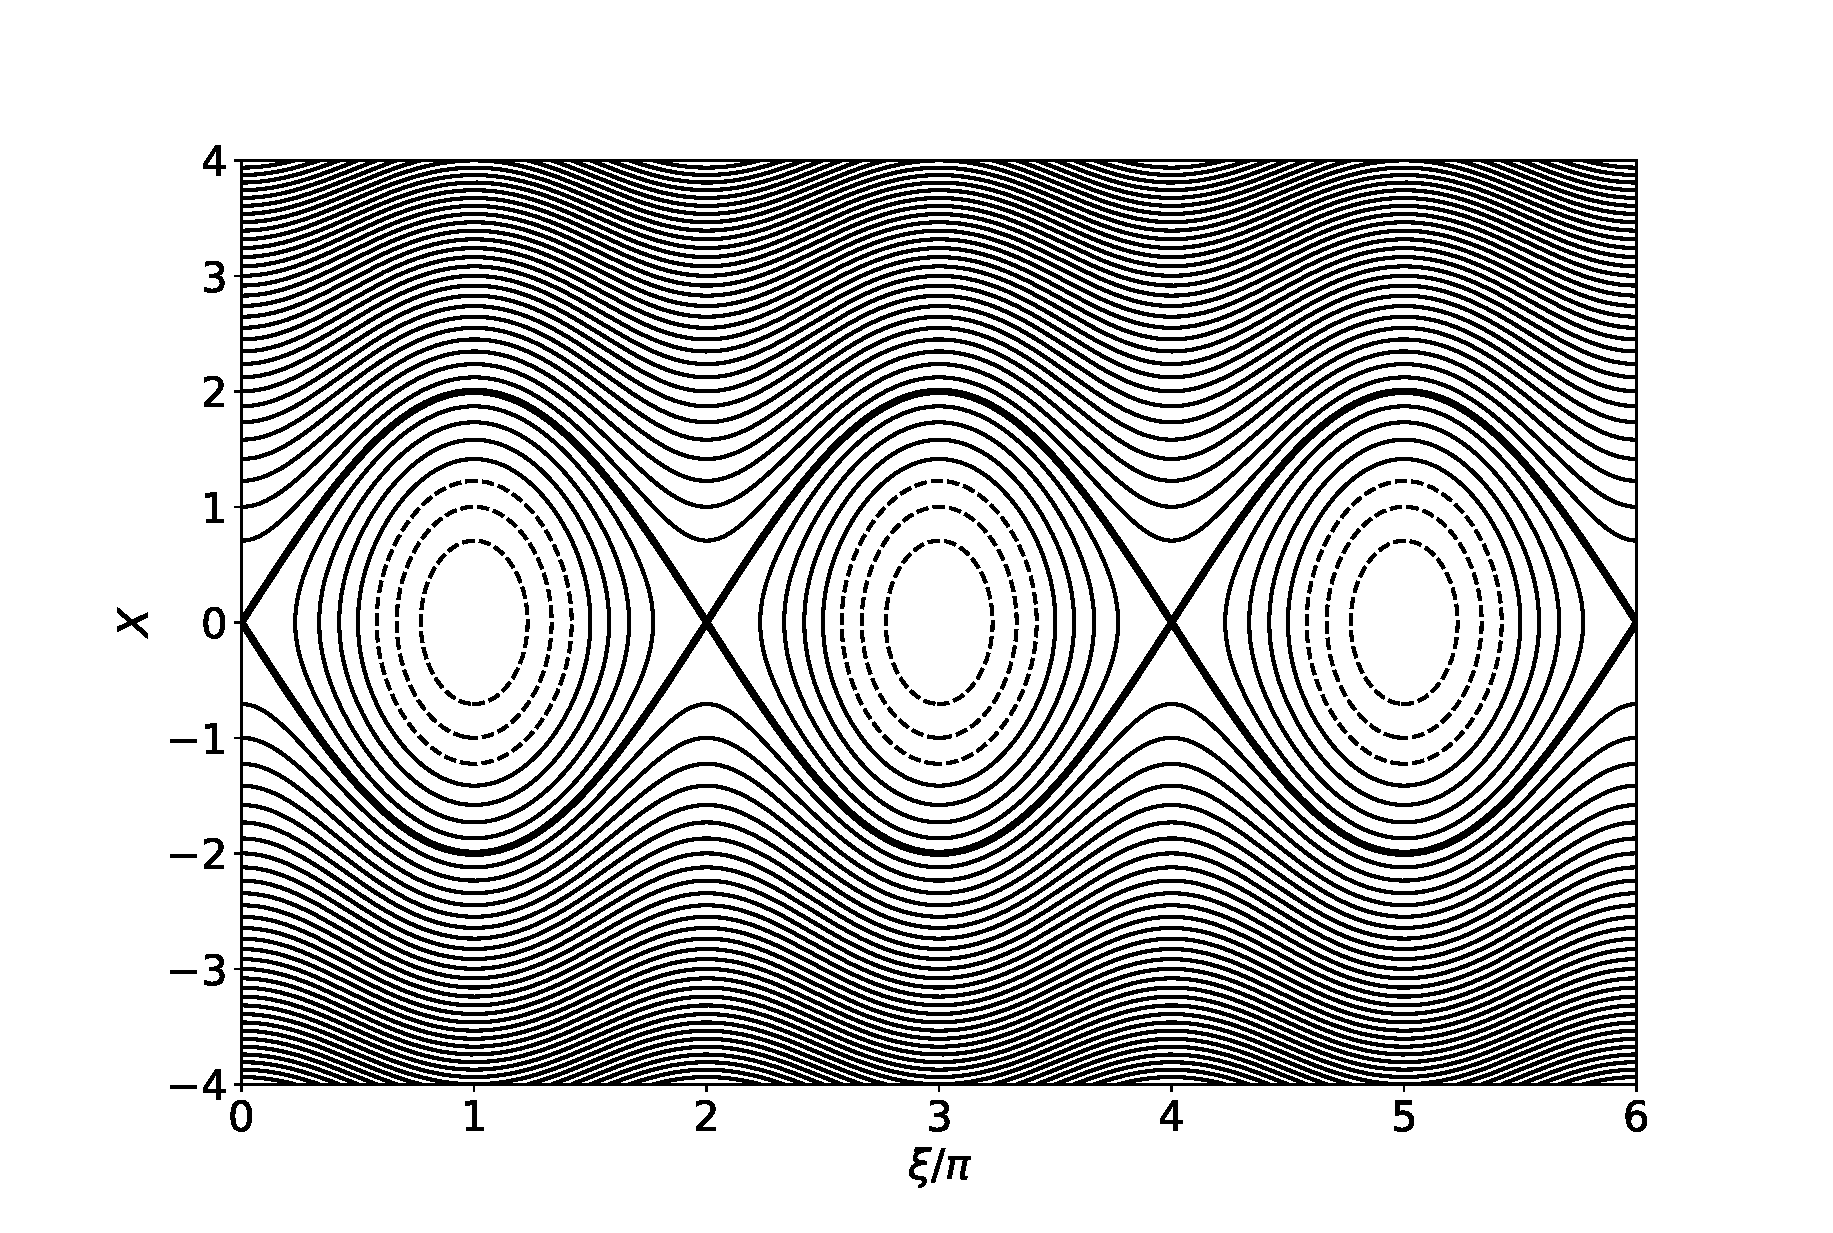
\includegraphics[height=4.5in]{Figure1.eps}}
\caption{Contours of the normalized magnetic flux, ${\mit\Omega}(X,\xi)$, in the one-harmonic approximation. Positive/negative contours are shown as solid/dashed lines. The magnetic separatrix is shown
as a  bold line.}\label{fig1}
\end{figure}

\begin{figure}
\centerline{\includegraphics[height=4.5in]{Figure2.eps}}
\caption{The current-drive function, $K_1(p_c)$, evaluated in the one-harmonic approximation.}\label{fig2}
\end{figure}

\begin{figure}
\centerline{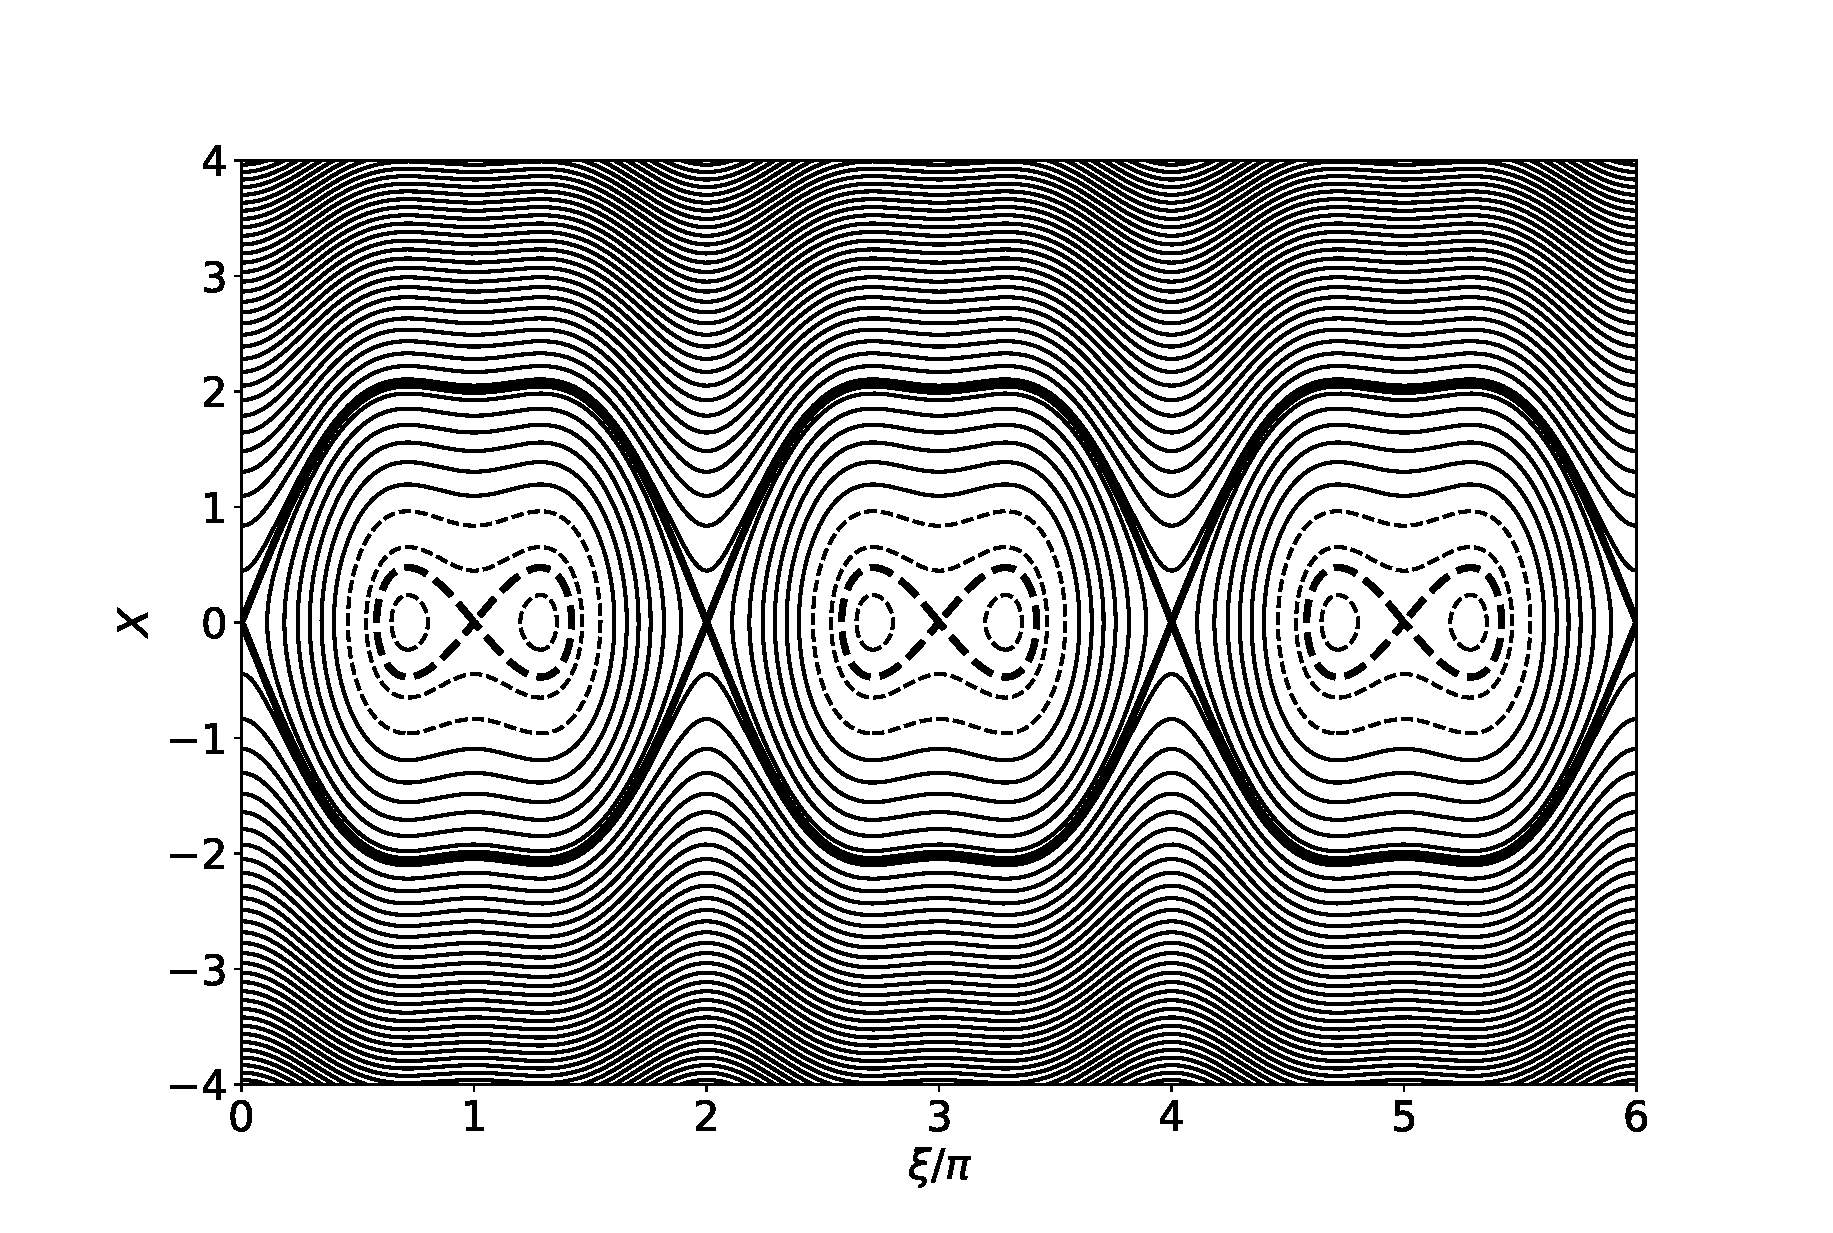
\includegraphics[height=4.5in]{Figure3.eps}}
\caption{ Contours of the normalized magnetic flux, ${\mit\Omega}(X,\xi)$, in the two-harmonic approximation for 
$\epsilon_2=0.4$. Positive/negative contours are shown as solid/dashed lines. The magnetic separatrices are shown
as  bold lines.}\label{fig3}
\end{figure}

\begin{figure}
\centerline{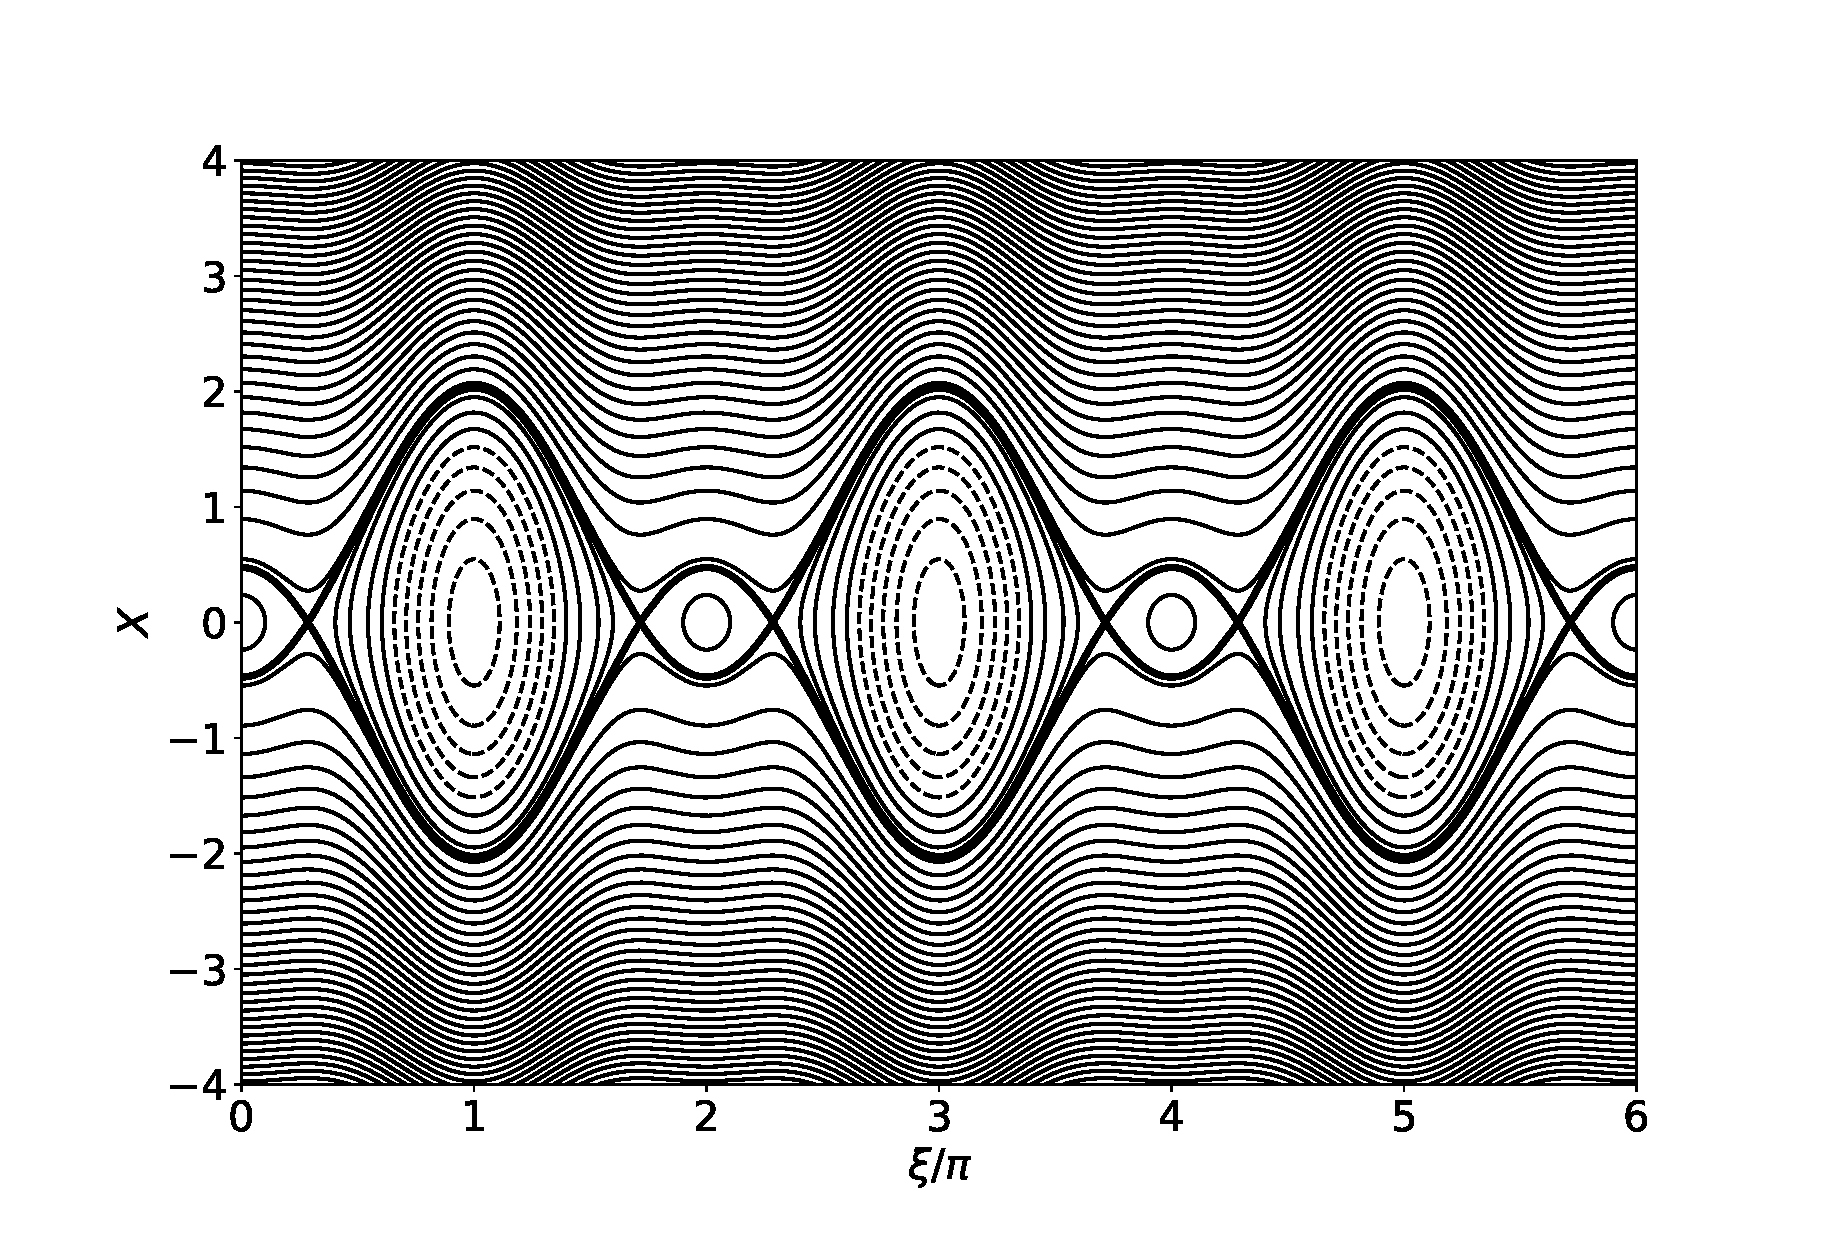
\includegraphics[height=4.5in]{Figure4.eps}}
\caption{ Contours of the normalized magnetic flux, ${\mit\Omega}(X,\xi)$, in the two-harmonic approximation for 
$\epsilon_2=-0.4$. Positive/negative contours are shown as solid/dashed lines. The magnetic separatrix is shown
as a  bold line.}\label{fig4}
\end{figure}

\begin{figure}
\centerline{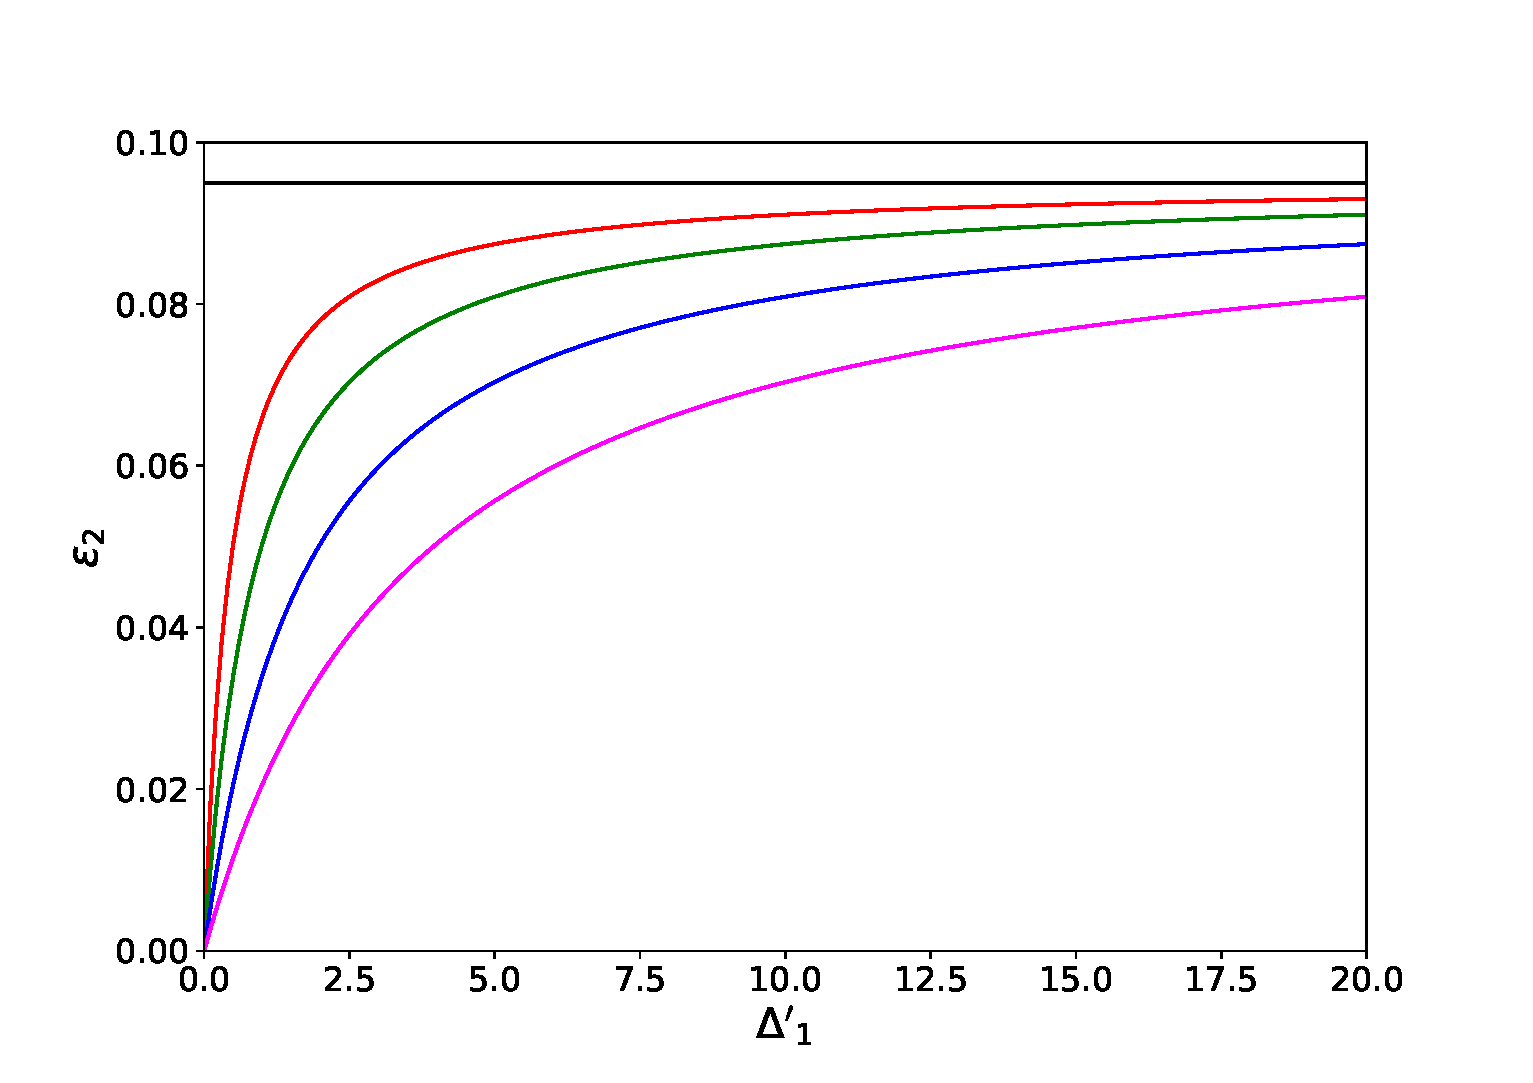
\includegraphics[height=4.5in]{Figure5.eps}}
\caption{$\epsilon_2$ versus ${\mit\Delta}_1'$, in the two-harmonic approximation, for a classical
tearing mode in the absence of RF-driven non-inductive current. The black, red,
green, blue, and magenta curves corresponds  to ${\mit\Delta}_2'=0.0$, $-0.5$,
$-1.0$, $-2.0$, and $-4.0$, respectively. }\label{fig5}
\end{figure}

\begin{figure}
\centerline{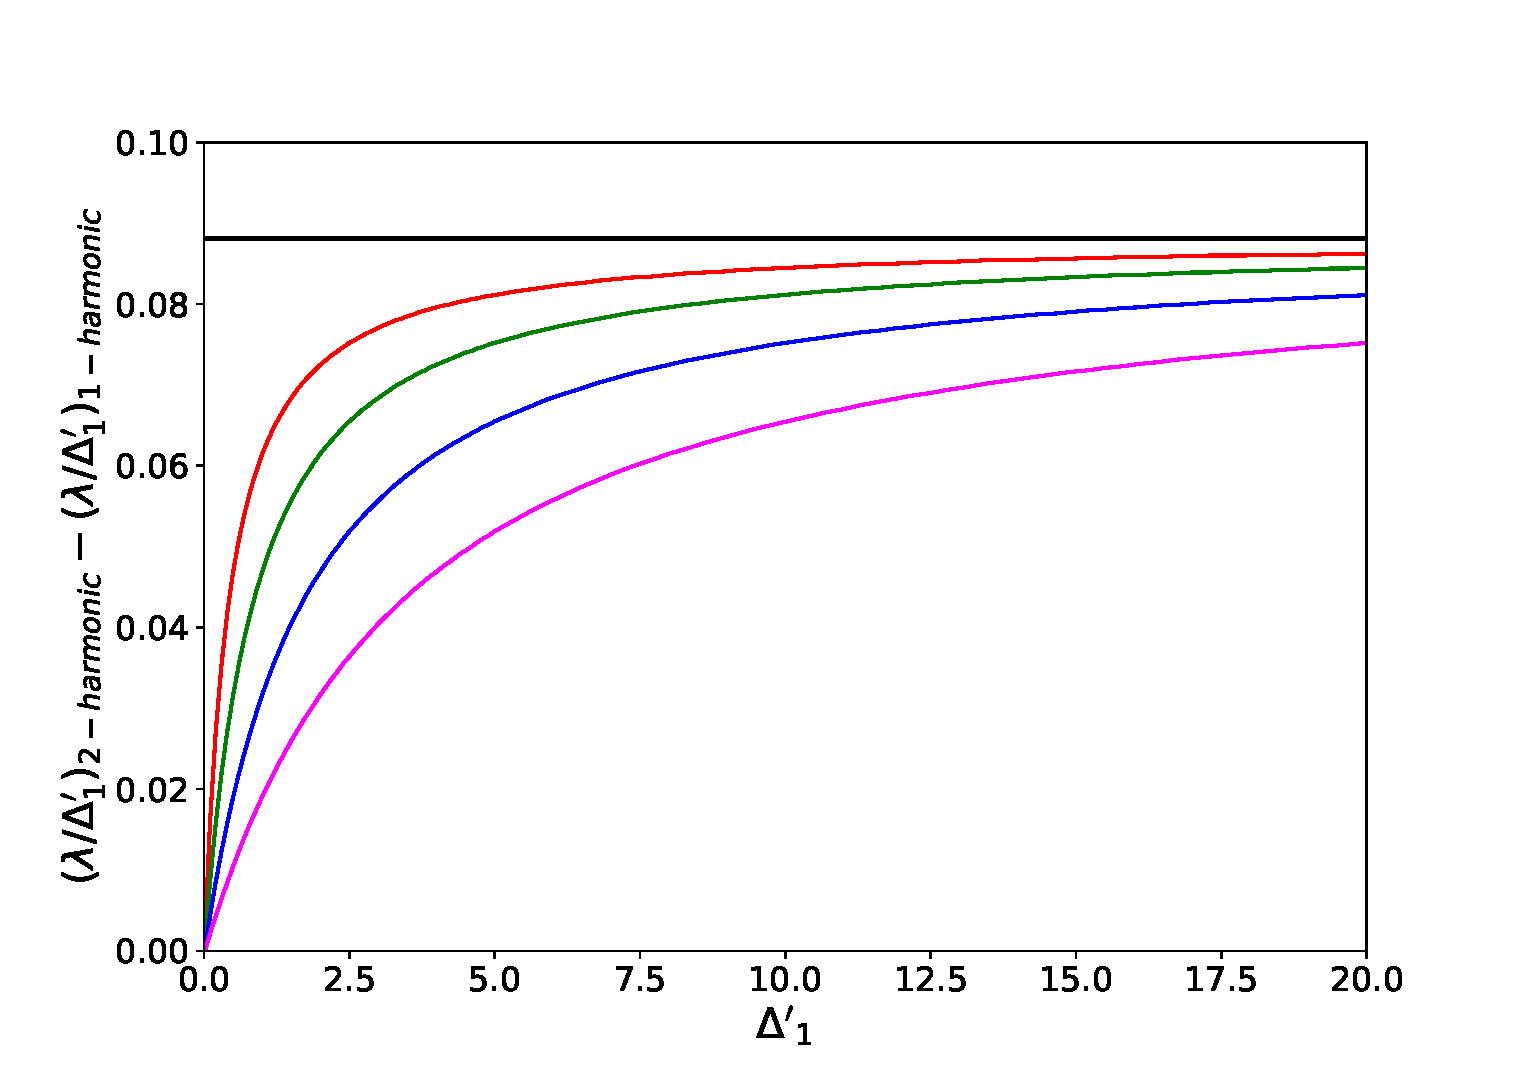
\includegraphics[height=4.5in]{Figure6.eps}}
\caption{Difference between $\lambda/{\mit\Delta}_1'$ in the two- and one-harmonic approximations for a classical
tearing mode in the absence of RF-driven non-inductive current. The black, red,
green, blue, and magenta curves corresponds  to ${\mit\Delta}_2'=0.0$, $-0.5$,
$-1.0$, $-2.0$, and $-4.0$, respectively. }\label{fig6}
\end{figure}

\begin{figure}
\centerline{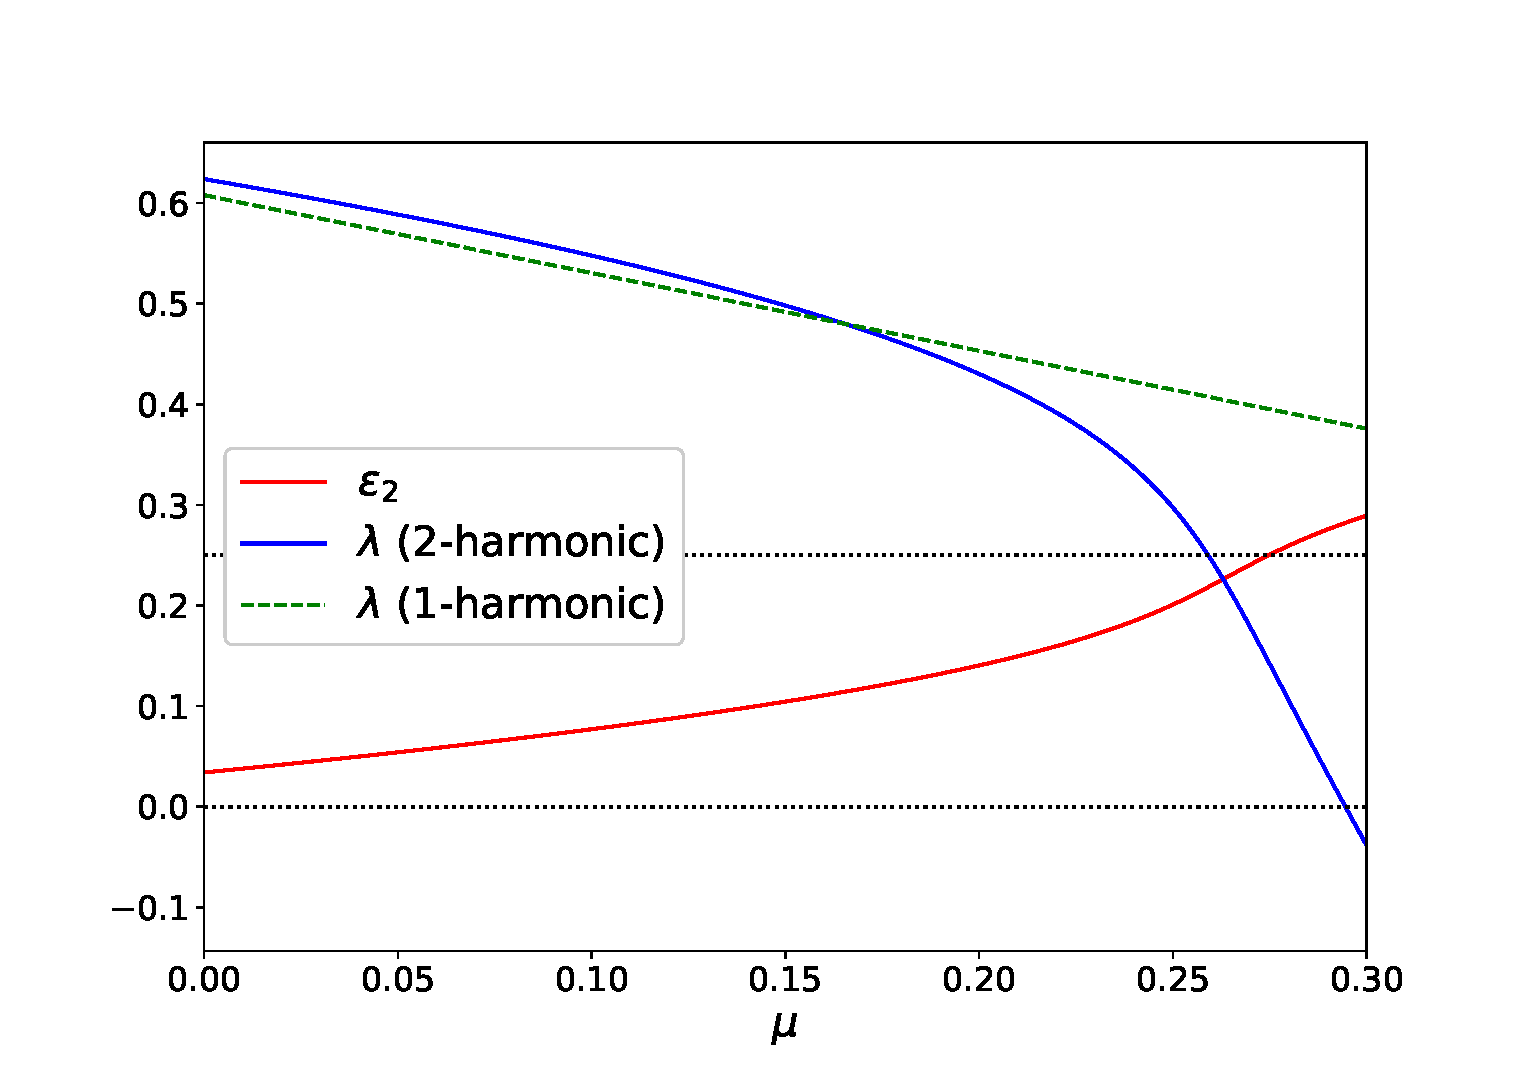
\includegraphics[height=4.5in]{Figure7.eps}}
\caption{Stabilization of a classical tearing mode by RF-driven non-inductive current in two- and one-harmonic approximations. The
calculation is performed with $p_c=0.2$, ${\mit\Delta}_1'=0.5$, and ${\mit\Delta}_2'=-1.0$.  }\label{fig7}
\end{figure}

\begin{figure}
\centerline{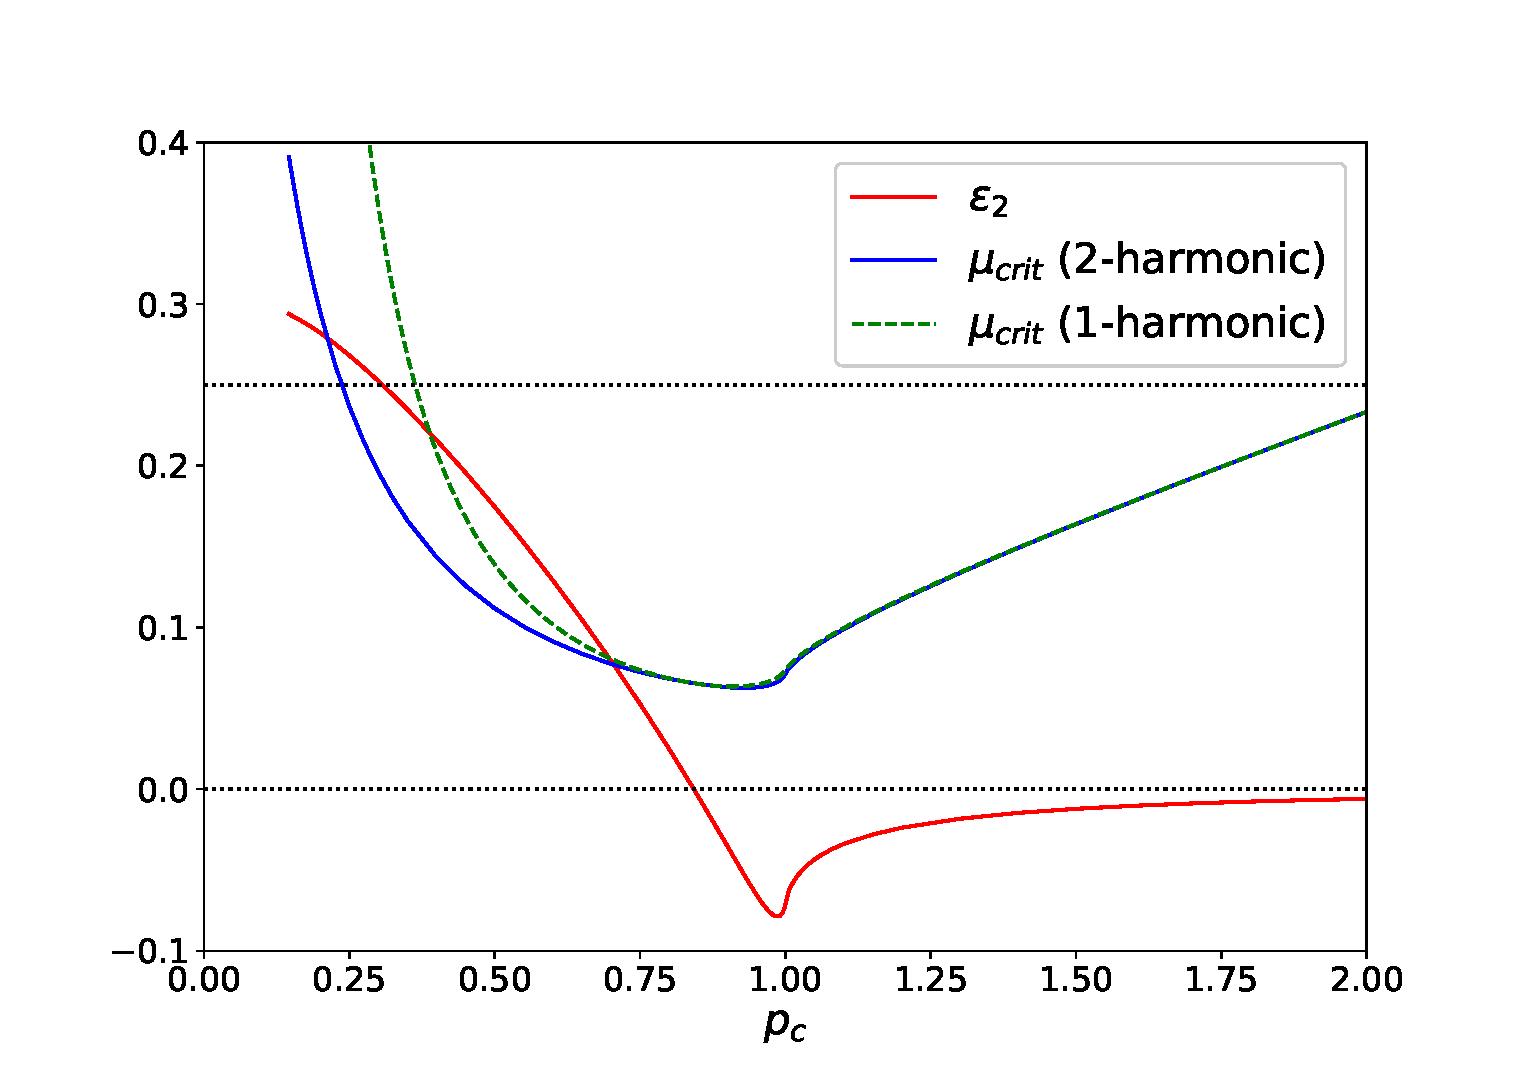
\includegraphics[height=4.5in]{Figure8.eps}}
\caption{Critical non-inductive RF-current drive parameter, $\mu$, needed to stabilize a classical tearing mode,  in the two- and one-harmonic approximations, as a function of the injection width parameter, $p_c$. The
calculation is performed with ${\mit\Delta}_1'=0.5$, and ${\mit\Delta}_2'=-1.0$.  }\label{fig8}
\end{figure}

\end{document}